% !Mode:: "TeX:UTF-8"
% 第二版:增加一个坐标变换的例子
\chapter{三维空间刚体运动}
\label{cpt:3}
\begin{mdframed}  
	\textbf{主要目标}
	\begin{enumerate}[labelindent=0em,leftmargin=1.5em]
		\item 理解三维空间的刚体运动描述方式:旋转矩阵、变换矩阵、四元数和欧拉角。
		\item 掌握Eigen库的矩阵、几何模块使用方法。
	\end{enumerate}
\end{mdframed} 

在上一讲中,我们讲解了视觉SLAM的框架与内容。本讲将介绍视觉SLAM的基本问题之一:\textbf{如何描述刚体在三维空间中的运动}?直观上看,我们当然知道这由一次旋转加一次平移组成。平移确实没有太大问题,但旋转的处理是件麻烦事。我们将介绍旋转矩阵、四元数、欧拉角的意义,以及它们是如何运算和转换的。在实践部分,我们将介绍线性代数库Eigen。它提供了C++中的矩阵运算,并且它的Geometry模块还提供了四元数等描述刚体运动的结构。Eigen的优化非常完善,但是它的使用方法有一些特殊的地方,我们留到程序中介绍。

\newpage
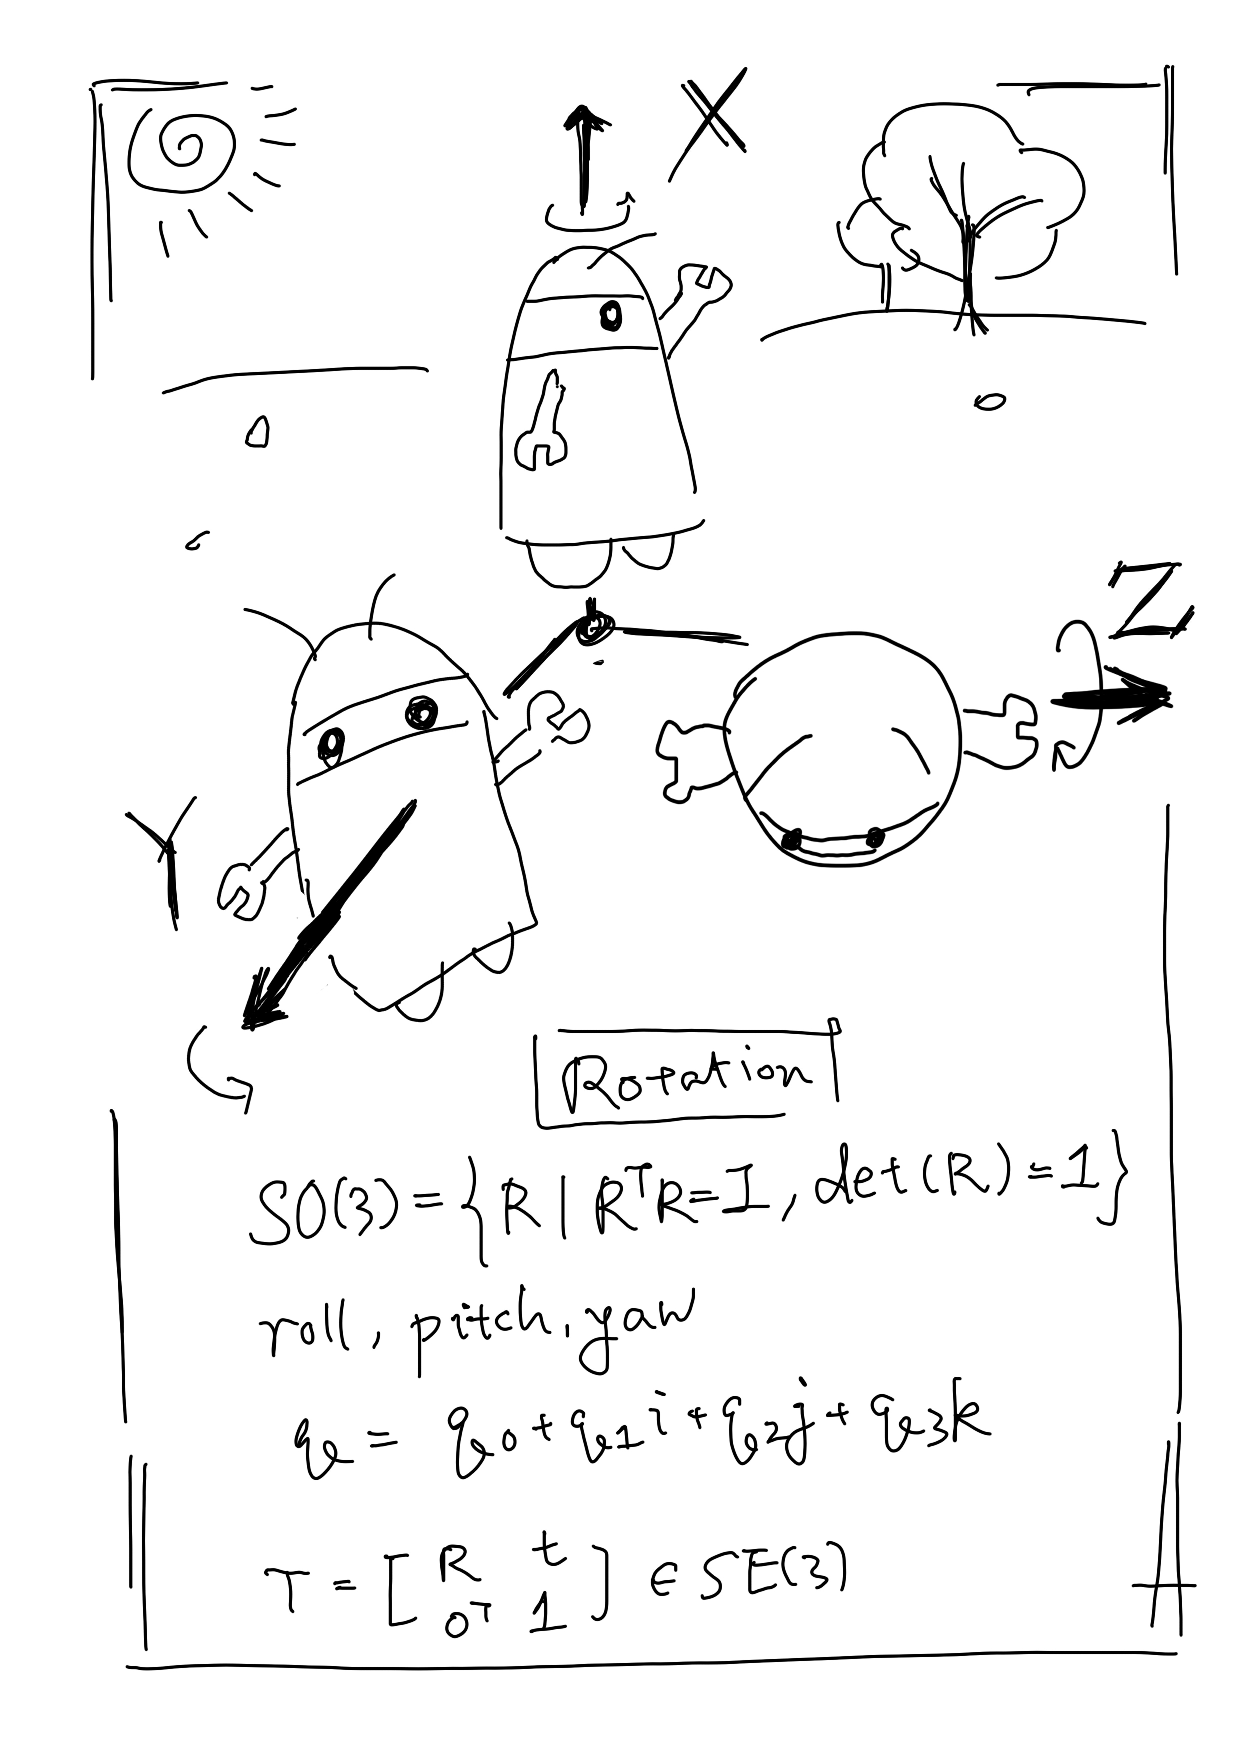
\includepdf{resources/other/ch3.pdf}

\newpage

\section{旋转矩阵}
\label{sec:rigidMotion}
\subsection{点和向量,坐标系}
我们日常生活的空间是三维的,因此我们生来就习惯于三维空间的运动。三维空间由3个轴组成,所以一个空间点的位置可以由3个坐标指定。不过,我们现在要考虑\textbf{刚体},它不光有位置,还有自身的姿态。相机也可以看成三维空间的刚体,于是位置是指相机在空间中的哪个地方,而姿态则是指相机的朝向。结合起来,我们可以说,“相机正处于空间$(0,0,0)$点处,朝向正前方”这样的话。但是这种自然语言很烦琐,我们更喜欢用数学语言来描述它。

我们从最基本的内容讲起:\textbf{点}和\textbf{向量}。点就是空间当中的基本元素,没有长度,没有体积。把两个点连接起来,就构成了向量。向量可以看成从某点指向另一点的一个箭头。需要提醒读者的是,请不要把向量与它的\textbf{坐标}两个概念混淆。一个向量是空间当中的一样东西,比如说$\bm{a}$。这里$\bm{a}$并不需要和若干个实数相关联的。只有当我们指定这个三维空间中的某个\textbf{坐标系}时,才可以谈论该向量在此坐标系下的坐标,也就是找到若干个实数对应这个向量。

用线性代数的知识来说,三维空间中的某个点的坐标也可以用$\mathbb{R}^3$来描述。怎么描述呢?假设在这个线性空间内,我们找到了该空间的一组\textbf{基}\footnote{以防读者忘记,基就是张成这个空间的一组线性无关的向量,有些书里也叫\textbf{基底}。}$(\bm{e}_1,\bm{e}_2,\bm{e}_3)$,那么,任意向量$\bm{a}$在这组基下就有一个\textbf{坐标}:
\begin{equation}
\bm{a} = \left[ {{\bm{e}_1},{\bm{e}_2},{\bm{e}_3}} \right]\left[ \begin{array}{l}
{a_1}\\
{a_2}\\
{a_3}
\end{array} \right] = {a_1}{\bm{e}_1} + {a_2}{\bm{e}_2} + {a_3}{\bm{e}_3}.
\end{equation}
这里$(a_1,a_2,a_3)^\mathrm{T}$称为$\bm{a}$在此基下的坐标\footnote{本书的向量为列向量,这和一般的数学书籍类似。}。坐标的具体取值,一是和向量本身有关,二是和坐标系(基)的选取有关。坐标系通常由3个正交的坐标轴组成(尽管也可以有非正交的,但实际中很少见)。例如,给定$\bm{x}$和$\bm{y}$轴时,$\bm{z}$轴就可以通过右手(或左手)法则由$\bm{x} \times \bm{y}$定义出来。根据定义方式的不同,坐标系又分为左手系和右手系。左手系的第3个轴与右手系方向相反。大部分3D程序库使用右手系(如OpenGL,3D Max等),也有部分库使用左手系(如Unity,Direct3D等)。

根据基本的线性代数知识,我们可以谈论向量与向量,以及向量与数之间的运算,例如数乘、加法、减法、内积、外积等。数乘和加减法都是相当基本的内容,也符合直观想象。例如,两个向量相加的结果就是把它们各自坐标相加,减法亦然,等等。这里不再赘述。内外积对读者来说可能有些陌生,这里给出它们的运算方式。对于$\bm{a}, \bm{b} \in \mathbb{R}^3$,通常意义下\footnote{内积也有形式化的法则,但本书只讨论通常的内积。}的内积可以写成:
\begin{equation}
\bm{a} \cdot \bm{b} = { \bm{a}^\mathrm{T}}\bm{b} = \sum\limits_{i = 1}^3 {{a_i}{b_i}}  = \left| \bm{a} \right|\left| \bm{b} \right|\cos \left\langle {\bm{a},\bm{b}} \right\rangle .
\end{equation}
其中$\left\langle {\bm{a},\bm{b}} \right\rangle$指向量$\bm{a},\bm{b}$的夹角。内积也可以描述向量间的投影关系。而外积则是这个样子:
\begin{equation}
\label{eq:cross}
\bm{a} \times \bm{b} = \left\| {\begin{array}{*{20}{c}}
	\bm{e}_1 & \bm{e}_2 & \bm{e}_3 \\
	{{a_1}}&{{a_2}}&{{a_3}}\\
	{{b_1}}&{{b_2}}&{{b_3}}
	\end{array}} \right\| = \left[ \begin{array}{l}
{a_2}{b_3} - {a_3}{b_2}\\
{a_3}{b_1} - {a_1}{b_3}\\
{a_1}{b_2} - {a_2}{b_1}
\end{array} \right] = \left[ {\begin{array}{*{20}{c}}
	0&{ - {a_3}}&{{a_2}}\\
	{{a_3}}&0&{ - {a_1}}\\
	{ - {a_2}}&{{a_1}}&0
	\end{array}} \right] \bm{b} \buildrel \Delta \over = { \bm{a}^ \wedge } \bm{b}.
\end{equation}

外积的结果是一个向量,它的方向垂直于这两个向量,大小为 $\left| \bm{a} \right|\left| \bm{b} \right|\sin \left\langle {\bm{a},\bm{b}} \right\rangle $,是两个向量张成的四边形的有向面积。对于外积运算,我们引入$^ \wedge$符号,把$\bm{a}$写成一个矩阵。事实上是一个\textbf{反对称矩阵}(Skew-symmetric matrix)\footnote{反对称矩阵$\bm{A}$满足$\bm{A}^\mathrm{T}=-\bm{A}$。},你可以将$^ \wedge$记成一个反对称符号。这样就把外积$\bm{a} \times \bm{b}$写成了矩阵与向量的乘法${ \bm{a}^ \wedge } \bm{b}$,把它变成了线性运算。这个符号将在后文经常用到,请记住它,并且此符号是一个一一映射,意味着任意向量都对应着唯一的一个反对称矩阵,反之亦然:
\begin{equation}
\bm{a}^\wedge = \left[ {\begin{array}{*{20}{c}}
	0&{ - {a_3}}&{{a_2}}\\
	{{a_3}}&0&{ - {a_1}}\\
	{ - {a_2}}&{{a_1}}&0
	\end{array}} \right].
\end{equation}

同时,需要提醒读者的是,向量和加减法、内外积,即使在不谈论它们的坐标时也可以计算。例如,虽然内积在有坐标时,可以用两个向量的分量乘积之和表达,但是即使不知道它们的坐标时,也可以通过长度和夹角来计算二者的内积。所以两个向量的内积结果和坐标系的选取是无关的。

%我们还能用外积表示向量的\textbf{旋转}。
%
%为什么外积可以表示旋转呢?
%
%考虑两个不平行的向量$\bm{a}, \bm{b}$,我们要描述从$\bm{a}$到$\bm{b}$之间是如何旋转的,如\autoref{fig:rotationOfVector}所示。我们可以用一个向量来描述三维空间中两个向量的旋转关系。在右手法则下,我们用右手的4个指头从$\bm{a}$转向$\bm{b}$,大拇指朝向就是旋转向量的方向,事实上也是$\bm{a} \times \bm{b}$的方向。它的大小则由$\bm{a}$和$\bm{b}$的夹角决定。通过这种方式,我们构造了从$\bm{a}$到$\bm{b}$的一个旋转向量。这个向量同样位于三维空间中,在此坐标系下,可以用3个实数来描述。
%
%\begin{figure}[!htp]
%	\centering
%	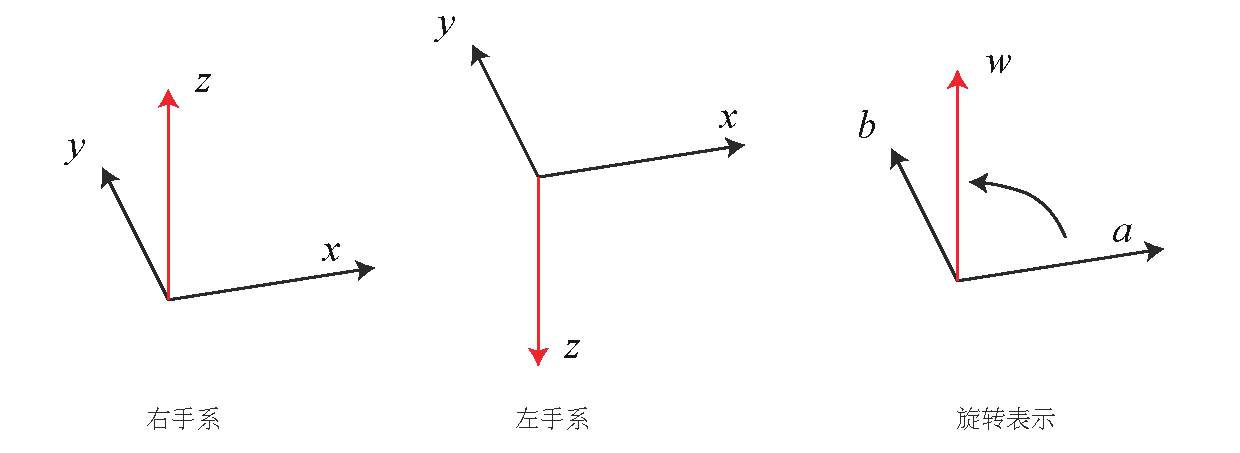
\includegraphics[width=1.0\textwidth]{rigidMotion/axis.pdf}
%	\caption{左右手系的区别与向量间的旋转。$\bm{a}$到$\bm{b}$的旋转可以由向量$\bm{w}$来描述。}
%	\label{fig:rotationOfVector}
%\end{figure}

\subsection{坐标系间的欧氏变换}
我们经常会在实际场景中定义各种各样的坐标系。在机器人学中,你会给每一个连杆和关节都定义它们的坐标系;在3D作图时,我们也会定义每一个长方体、圆柱体的坐标系。如果考虑运动的机器人,那么常见的做法是设定一个惯性坐标系(或者叫世界坐标系),可以认为它是固定不动的,例如\autoref{fig:axisTransform}中的$x_W, y_W, z_W$定义的坐标系。同时,相机或机器人则是一个移动坐标系,例如$x_C, y_C, z_C$定义的坐标系。我们可能会问:相机视野中某个向量$\bm{p}$,它在相机坐标系下的坐标为$\bm{p}_c$,而在世界坐标系下看,它的坐标为$\bm{p}_w$,那么,这两个坐标之间是如何转换的呢?这时,就需要先得到该点针对机器人坐标系的坐标值,再根据机器人位姿\textbf{变换}到世界坐标系中。我们需要一种数学手段来描述这个变换关系,稍后我们会看到,可以用一个矩阵$\bm{T}$来描述它。

\begin{figure}[!htp]
	\centering
	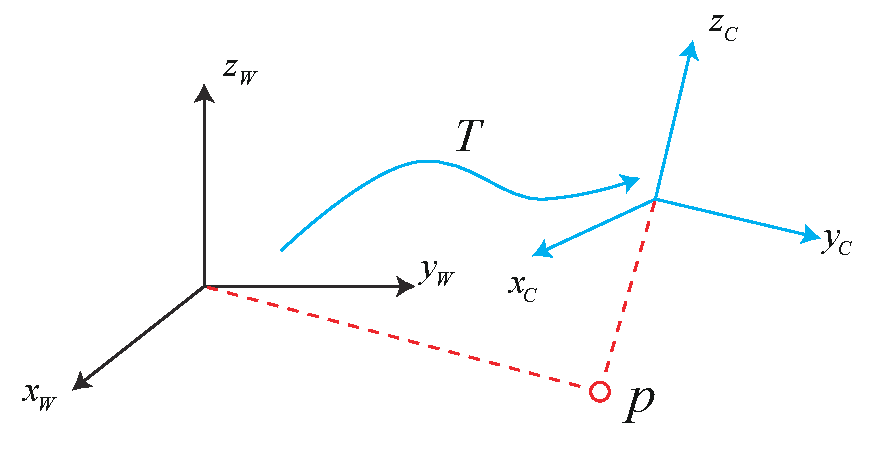
\includegraphics[width=0.7\textwidth]{rigidMotion/axisTransform.pdf}
	\caption{坐标变换。对于同一个向量$\bm{p}$,它在世界坐标系下的坐标$\bm{p}_w$和在相机坐标系下的坐标$\bm{p}_c$是不同的。这个变换关系由变换矩阵$\bm{T}$来描述。}
	\label{fig:axisTransform}
\end{figure}

直观上看,两个坐标系之间的运动由一个旋转加上一个平移组成,这种运动称为\textbf{刚体运动}。相机运动就是一个刚体运动。刚体运动过程中,同一个向量在各个坐标系下的长度和夹角都不会发生变化。想象你把手机抛到空中,在它落地摔碎之前\footnote{请不要付诸实践。},只可能有空间位置和姿态的不同,而它自己的长度、各个面的角度等性质不会有任何变化。手机并不会像橡皮那样一会儿被挤扁,一会儿被拉长。此时,我们说手机坐标系到世界坐标之间,相差了一个\textbf{欧氏变换}(Euclidean Transform)。

欧氏变换由旋转和平移组成。我们首先考虑旋转。设某个单位正交基$(\bm{e}_1,\bm{e}_2,\bm{e}_3)$经过一次旋转变成了$(\bm{e}_1', \bm{e}_2', \bm{e}_3')$。那么,对于同一个向量$\bm{a}$(该向量并没有随着坐标系的旋转而发生运动),它在两个坐标系下的坐标为$[a_1,a_2,a_3]^\mathrm{T}$和$[a'_1, a'_2, a'_3]^\mathrm{T}$。因为向量本身没变,根据坐标的定义,有:

\begin{equation}
\left[ \bm{e}_1,\bm{e}_2,\bm{e}_3 \right]\left[ \begin{array}{l}
{a_1}\\
{a_2}\\
{a_3}
\end{array} \right] = \left[ \bm{e}_1', \bm{e}_2', \bm{e}_3' \right]\left[ \begin{array}{l}
a'_1\\
a'_2\\
a'_3
\end{array} \right].
\end{equation}

为了描述两个坐标之间的关系,我们对上述等式的左右两边同时左乘$\left[ \begin{array}{l}
\bm{e}_1^\mathrm{T}\\
\bm{e}_2^\mathrm{T}\\
\bm{e}_3^\mathrm{T}
\end{array} \right]$,那么左边的系数就变成了单位矩阵,所以:
%\clearpage
\begin{equation}
\left[ \begin{array}{l}
{a_1}\\
{a_2}\\
{a_3}
\end{array} \right] = \left[ {\begin{array}{*{20}{c}}
	{\bm{e}_1^\mathrm{T}\bm{e}_1'} & {\bm{e}_1^\mathrm{T}\bm{e}_2'} & {\bm{e}_1^\mathrm{T}\bm{e}_3'}\\
	{\bm{e}_2^\mathrm{T}\bm{e}_1'} & {\bm{e}_2^\mathrm{T}\bm{e}_2'} & {\bm{e}_2^\mathrm{T}\bm{e}_3'}\\
	{\bm{e}_3^\mathrm{T}\bm{e}_1'} & {\bm{e}_3^\mathrm{T}\bm{e}_2'} & {\bm{e}_3^\mathrm{T}\bm{e}_3'}
	\end{array}} \right]\left[ \begin{array}{l}
a_1'\\
a_2'\\
a_3'
\end{array} \right] \buildrel \Delta \over = \bm{R} \bm{a}'.
\end{equation}
我们把中间的矩阵拿出来,定义成一个矩阵$\bm{R}$。这个矩阵由两组基之间的内积组成,刻画了旋转前后同一个向量的坐标变换关系。只要旋转是一样的,那么这个矩阵也是一样的。可以说,矩阵$\bm{R}$描述了旋转本身。因此称为\textbf{旋转矩阵}(Rotation matrix)。同时,该矩阵各分量是两个坐标系基的内积,由于基向量的长度为1,所以实际上是各基向量的夹角之余弦。所以这个矩阵也叫\textbf{方向余弦矩阵}(Direction Cosine matrix)。我们后文统一称呼它为旋转矩阵。

旋转矩阵有一些特别的性质。事实上,它是一个行列式为1的正交矩阵\footnote{正交矩阵即逆为自身转置的矩阵。旋转矩阵的正交性可以直接由定义得出。}\footnote{行列式为1是人为定义的,实际上只要求它的行列式为$\pm 1$,但行列式为$-1$的称为瑕旋转,即一次旋转加一次反射。}。反之,行列式为1的正交矩阵也是一个旋转矩阵。所以,可以把$n$维旋转矩阵的集合定义如下:
\begin{equation}
\mathrm{SO}(n) = \{ \bm{R} \in \mathbb{R}^{n \times n} | \bm{R R}^\mathrm{T} = \bm{I}, \mathrm{det} (\bm{R})=1 \}.
\end{equation}

$\mathrm{SO}(n)$是\textbf{特殊正交群}(Special Orthogonal Group)的意思。我们把“群”的内容留到下一讲。这个集合由$n$维空间的旋转矩阵组成,特别地,$\mathrm{SO}(3)$就是指三维空间的旋转。通过旋转矩阵,我们可以直接谈论两个坐标系之间的旋转变换,而不用再从基开始谈起。

由于旋转矩阵为正交矩阵,它的逆(即转置)描述了一个相反的旋转。按照上面的定义方式,有:
\begin{equation}
\bm{a}' = \bm{R}^{-1} \bm{a} =\bm{R}^\mathrm{T} \bm{a} .
\end{equation}
显然$\bm{R}^\mathrm{T}$刻画了一个相反的旋转。

在欧氏变换中,除了旋转之外还有平移。考虑世界坐标系中的向量$\bm{a}$,经过一次旋转(用$\bm{R}$描述)和一次平移$\bm{t}$后,得到了$\bm{a}'$,那么把旋转和平移合到一起,有:
\begin{equation}
\label{eq:RT}
\bm{a}' = \bm{R} \bm{a} + \bm{t}.
\end{equation}
其中,$\bm{t}$称为平移向量。相比于旋转,平移部分只需把平移向量加到旋转之后的坐标上,非常简单。通过上式,我们用一个旋转矩阵$\bm{R}$和一个平移向量$\bm{t}$完整地描述了一个欧氏空间的坐标变换关系。实际当中,我们会定义坐标系1、坐标系2,那么向量$\bm{a}$在两个系下坐标为$\bm{a}_1, \bm{a}_2$,它们之间的关系,按照完整的写法,应该是:
\begin{equation}
\bm{a}_1 = \bm{R}_{12} \bm{a}_2 + \bm{t}_{12}.
\end{equation}
这里的$\bm{R}_{12}$是指“把坐标系2的向量变换到坐标系1”中。由于向量乘在这个矩阵的右边,它的下标是\textbf{从右读到左}的。这也是本书的习惯写法。坐标变换很容易搞混,特别是存在多个坐标系的情况下。同理,如果我们要表达“从1到2的旋转矩阵”时,就写成$\bm{R}_{21}$。请读者务必清楚这边的记法,因为不同书籍里写法不同,有的会记成左上/下标,而本书写在右侧下标。

关于平移$\bm{t}_{12}$,它实际对应的是坐标系1原点指向坐标系2原点的向量,\textbf{在坐标系1下取的坐标},所以我建议读者把它记作“从1到2的向量”。但是反过来的$\bm{t}_{21}$,即从2指向1的向量\textbf{在坐标系2下的坐标},却并不等于$-\bm{t}_{12}$,而是和两个系的旋转还有关系\footnote{尽管从向量层面来看,它们确实是反向的关系,但这两个向量的坐标值并不是相反数。你能想清楚这是为什么吗?}。所以,当初学者问“我的坐标在哪里”这样的问题时,我们需要清楚地说明这句话的含义。这里“我的坐标”实际上指从世界坐标系指向自己坐标系原点的向量,在世界坐标系下取到的坐标。对应到数学符号上,应该是$\bm{t}_{WC}$的取值。同理,它也不是$-\bm{t}_{CW}$。

\subsection{变换矩阵与齐次坐标}

式\eqref{eq:RT}完整地表达了欧氏空间的旋转与平移,不过还存在一个小问题:这里的变换关系不是一个线性关系。假设我们进行了两次变换:$\bm{R}_1,\bm{t}_1$和$\bm{R}_2,\bm{t}_2$:

\[
\bm{b} = {\bm{R}_1} \bm{a} + {\bm{t}_1}, \quad \bm{c} = {\bm{R}_2} \bm{b} + {\bm{t}_2}.
\]
那么,从$\bm{a}$到$\bm{c}$的变换为:
\[
\bm{c} = {\bm{R}_2}\left( {{\bm{R}_1} \bm{a} + {\bm{t}_1}} \right) + {\bm{t}_2}.
\]
这样的形式在变换多次之后会显得很啰嗦。因此,我们引入齐次坐标和变换矩阵,重写式\eqref{eq:RT}:
\begin{equation}
\left[ \begin{array}{l}
\bm{a}'\\
1
\end{array} \right] = 
\left[ {\begin{array}{*{20}{c}}
	\bm{R}&\bm{t}\\
	{{\bm{0}^\mathrm{T}}}&1
	\end{array}} \right]
\left[ \begin{array}{l}
\bm{a}\\
1
\end{array} \right]  \buildrel \Delta \over = \bm{T} \left[ \begin{array}{l}
\bm{a}\\
1
\end{array} \right].
\end{equation}

这是一个数学技巧:我们在一个三维向量的末尾添加$1$,将其变成了四维向量,称为\textbf{齐次坐标}。对于这个四维向量,我们可以把旋转和平移写在一个矩阵里面,使得整个关系变成线性关系。该式中,矩阵$\bm{T}$称为\textbf{变换矩阵(Transform Matrix)}。
%
%稍微说一下齐次坐标。它是射影几何里的概念。通过添加最后一维,我们用4个实数描述了一个三维向量,这显然多了一个自由度,但允许我们把变换写成线性的形式。在齐次坐标中,某个点$\bm{x}$的每个分量同乘一个非零常数$k$后,\textbf{仍然表示同一个点}。因此,一个点的具体坐标值不是唯一的。如$\left[1,1,1,1\right]^\mathrm{T}$和$\left[2,2,2,2\right]^\mathrm{T}$是同一个点。但当最后一项不为零时,我们总可以把所有坐标除以最后一项,强制最后一项为1,从而得到一个点唯一的坐标表示(也就是转换成非齐次坐标):
%\begin{equation}
%\tilde{\bm{x}} = \left[ x, y, z,w \right]^\mathrm{T} = \left[ x/w, y/w, z/w, 1 \right]^\mathrm{T} .
%\end{equation}
%
%这时,忽略掉最后一项,这个点的坐标和欧氏空间就是一样的。

我们暂时用$ \tilde{ \bm{a} }$表示$\bm{a}$的齐次坐标。那么依靠齐次坐标和变换矩阵,两次变换的叠加就可以有很好的形式:
\begin{equation}
	\tilde{\bm{b}} = \bm{T}_1 \tilde{\bm{a}}, \  \tilde{\bm{c}} = \bm{T}_2 \tilde{\bm{b}} \quad \Rightarrow \tilde{\bm{c}} = \bm{T}_2 \bm{T_1} \tilde{\bm{a}}.
\end{equation}
但是区分齐次和非齐次坐标的符号令我们感到厌烦,因为此处只需要在向量末尾添加1或者去掉1即可\footnote{但齐次坐标的用途不止于此,我们在第7章还会再介绍。}。所以,在不引起歧义的情况下,以后我们就直接把它写成$\bm{b}= \bm{T} \bm{a}$的样子,默认其中进行了齐次坐标的转换\footnote{注意,不进行齐次坐标转换时,这边的乘法在矩阵维度上是不成立的。}。

关于变换矩阵$\bm{T}$,它具有比较特别的结构:左上角为旋转矩阵,右侧为平移向量,左下角为$\bm{0}$向量,右下角为1。这种矩阵又称为特殊欧氏群(Special Euclidean Group):
\begin{equation}
\mathrm{SE}(3) = \left\{ \bm{T} = \left[ {\begin{array}{*{20}{c}}
	\bm{R} & \bm{t} \\
	{{\bm{0}^\mathrm{T}}} & 1
	\end{array}} \right]
\in \mathbb{R}^{4 \times 4} | \bm{R} \in \mathrm{SO}(3), \bm{t} \in \mathbb{R}^3\right\} .
\end{equation}

与$\mathrm{SO}(3)$一样,求解该矩阵的逆表示一个反向的变换:
\begin{equation}
{ \bm{T}^{ - 1}} = \left[ {\begin{array}{*{20}{c}}
	{{\bm{R}^\mathrm{T}}}&{ - {\bm{R}^\mathrm{T}}\bm{t}}\\
	{{\bm{0}^\mathrm{T}}}&1
	\end{array}} \right].
\end{equation}

同样,我们用$\bm{T}_{12}$这样的写法来表示从2到1的变换。并且,为了保持符号的简洁,在不引起歧义的情况下,以后不刻意区别齐次坐标与普通坐标的符号,\textbf{默认使用的是符合运算法则的那一种}。例如,当我们写$\bm{T} \bm{a}$时,使用的是齐次坐标(不然没法计算)。而写$\bm{Ra}$时,使用的是非齐次坐标。如果写在一个等式中,就假设齐次坐标到普通坐标的转换,是已经做好了的——因为齐次坐标和非齐次坐标之间的转换事实上非常容易,而在C++程序中你可以使用\textbf{运算符重载}来完成这个功能,保证在程序中看到的运算是统一的。

回顾一下:首先,我们介绍了向量及其坐标表示,并介绍了向量间的运算;然后,坐标系之间的运动由欧氏变换描述,它由平移和旋转组成。旋转可以由旋转矩阵$\mathrm{SO}(3)$描述,而平移直接由一个$\mathbb{R}^3$向量描述。最后,如果将平移和旋转放在一个矩阵中,就形成了变换矩阵$\mathrm{SE}(3)$。

\section{实践:Eigen}
本讲的实践部分有两节。第一部分中,将讲解如何使用Eigen来表示矩阵、向量,随后引申至旋转矩阵与变换矩阵的计算。本节的代码在slambook2/ch3/useEigen中。

Eigen\footnote{官方主页:\url{http://eigen.tuxfamily.org/index.php?title=Main_Page}。}是一个C++开源线性代数库。它提供了快速的有关矩阵的线性代数运算,还包括解方程等功能。许多上层的软件库也使用Eigen进行矩阵运算,包括g2o、Sophus等。照应本讲的理论部分,我们来学习一下Eigen的编程。

你的PC上可能还没有安装Eigen。请输入以下命令进行安装:
\begin{lstlisting}[language=sh,caption=终端输入:]
sudo apt-get install libeigen3-dev
\end{lstlisting}

大部分常用的库都已在Ubuntu软件源中提供。以后,若想要安装某个库,不妨先搜索一下Ubuntu的软件源中是否已提供。通过apt命令,我们能够方便地安装Eigen。回顾上一讲的知识,我们知道一个库由头文件和库文件组成。Eigen头文件的默认位置在“/usr/include/eigen3/”中。如果不确定,可以输入以下命令查找:
\begin{lstlisting}[language=sh,caption=终端输入:]
sudo updatedb
locate eigen3
\end{lstlisting}
相比于其他库,Eigen的特殊之处在于,它是一个纯用头文件搭建起来的库(这非常神奇!)。这意味着你只能找到它的头文件,而没有.so或.a那样的二进制文件。在使用时,只需引入Eigen的头文件即可,不需要链接库文件(因为它没有库文件)。下面写一段代码来实际练习一下Eigen的使用:

\begin{lstlisting}[language=c++,caption=slambook2/ch3/useEigen/eigenMatrix.cpp]
#include <iostream>
using namespace std;

#include <ctime>
// Eigen 核心部分
#include <Eigen/Core>
// 稠密矩阵的代数运算(逆,特征值等)
#include <Eigen/Dense>
using namespace Eigen;

#define MATRIX_SIZE 50

/****************************
* 本程序演示了 Eigen 基本类型的使用
****************************/

int main(int argc, char **argv) {
	// Eigen 中所有向量和矩阵都是Eigen::Matrix,它是一个模板类。它的前三个参数为:数据类型,行,列
	// 声明一个2*3的float矩阵
	Matrix<float, 2, 3> matrix_23;
	
	// 同时,Eigen 通过 typedef 提供了许多内置类型,不过底层仍是Eigen::Matrix
	// 例如 Vector3d 实质上是 Eigen::Matrix<double, 3, 1>,即三维向量
	Vector3d v_3d;
	// 这是一样的
	Matrix<float, 3, 1> vd_3d;
	
	// Matrix3d 实质上是 Eigen::Matrix<double, 3, 3>
	Matrix3d matrix_33 = Matrix3d::Zero(); //初始化为零
	// 如果不确定矩阵大小,可以使用动态大小的矩阵
	Matrix<double, Dynamic, Dynamic> matrix_dynamic;
	// 更简单的
	MatrixXd matrix_x;
	// 这种类型还有很多,我们不一一列举
	
	// 下面是对Eigen阵的操作
	// 输入数据(初始化)
	matrix_23 << 1, 2, 3, 4, 5, 6;
	// 输出
	cout << "matrix 2x3 from 1 to 6: \n" << matrix_23 << endl;
	
	// 用()访问矩阵中的元素
	cout << "print matrix 2x3: " << endl;
	for (int i = 0; i < 2; i++) {
		for (int j = 0; j < 3; j++) cout << matrix_23(i, j) << "\t";
		cout << endl;
	}
	
	// 矩阵和向量相乘(实际上仍是矩阵和矩阵)
	v_3d << 3, 2, 1;
	vd_3d << 4, 5, 6;
	
	// 但是在Eigen里你不能混合两种不同类型的矩阵,像这样是错的
	// Matrix<double, 2, 1> result_wrong_type = matrix_23 * v_3d;
	// 应该显式转换
	Matrix<double, 2, 1> result = matrix_23.cast<double>() * v_3d;
	cout << "[1,2,3;4,5,6]*[3,2,1]=" << result.transpose() << endl;
	
	Matrix<float, 2, 1> result2 = matrix_23 * vd_3d;
	cout << "[1,2,3;4,5,6]*[4,5,6]: " << result2.transpose() << endl;
	
	// 同样你不能搞错矩阵的维度
	// 试着取消下面的注释,看看Eigen会报什么错
	// Eigen::Matrix<double, 2, 3> result_wrong_dimension = matrix_23.cast<double>() * v_3d;
	
	// 一些矩阵运算
	// 四则运算就不演示了,直接用+-*/即可。
	matrix_33 = Matrix3d::Random();      // 随机数矩阵
	cout << "random matrix: \n" << matrix_33 << endl;
	cout << "transpose: \n" << matrix_33.transpose() << endl; // 转置
	cout << "sum: " << matrix_33.sum() << endl;               // 各元素和
	cout << "trace: " << matrix_33.trace() << endl;           // 迹
	cout << "times 10: \n" << 10 * matrix_33 << endl;         // 数乘
	cout << "inverse: \n" << matrix_33.inverse() << endl;     // 逆
	cout << "det: " << matrix_33.determinant() << endl;       // 行列式
	
	// 特征值
	// 实对称矩阵可以保证对角化成功
	SelfAdjointEigenSolver<Matrix3d> eigen_solver(matrix_33.transpose() * matrix_33);
	cout << "Eigen values = \n" << eigen_solver.eigenvalues() << endl;
	cout << "Eigen vectors = \n" << eigen_solver.eigenvectors() << endl;
	
	// 解方程
	// 我们求解 matrix_NN * x = v_Nd 这个方程
	// N的大小在前边的宏里定义,它由随机数生成
	// 直接求逆自然是最直接的,但是求逆运算量大
	
	Matrix<double, MATRIX_SIZE, MATRIX_SIZE> matrix_NN
		= MatrixXd::Random(MATRIX_SIZE, MATRIX_SIZE);
	matrix_NN = matrix_NN * matrix_NN.transpose();  // 保证半正定
	Matrix<double, MATRIX_SIZE, 1> v_Nd = MatrixXd::Random(MATRIX_SIZE, 1);
	
	clock_t time_stt = clock(); // 计时
	// 直接求逆
	Matrix<double, MATRIX_SIZE, 1> x = matrix_NN.inverse() * v_Nd;
	cout << "time of normal inverse is "
	     << 1000 * (clock() - time_stt) / (double) CLOCKS_PER_SEC << "ms" << endl;
	cout << "x = " << x.transpose() << endl;
	
	// 通常用矩阵分解来求,例如QR分解,速度会快很多
	time_stt = clock();
	x = matrix_NN.colPivHouseholderQr().solve(v_Nd);
	cout << "time of Qr decomposition is "
	     << 1000 * (clock() - time_stt) / (double) CLOCKS_PER_SEC << "ms" << endl;
	cout << "x = " << x.transpose() << endl;
	
	// 对于正定矩阵,还可以用cholesky分解来解方程
	time_stt = clock();
	x = matrix_NN.ldlt().solve(v_Nd);
	cout << "time of ldlt decomposition is "
	     << 1000 * (clock() - time_stt) / (double) CLOCKS_PER_SEC << "ms" << endl;
	cout << "x = " << x.transpose() << endl;
	
	return 0;
}
\end{lstlisting}

这个例程演示了Eigen矩阵的基本操作与运算。要编译它,需要在CMakeLists.txt里指定Eigen的头文件目录:
\begin{lstlisting}[caption=slambook2/ch3/useEigen/CMakeLists.txt]
# 添加头文件
include_directories( "/usr/include/eigen3" )
\end{lstlisting}

重复一遍,因为Eigen库只有头文件,所以不需要再用target\_link\_libraries语句将程序链接到库上。不过,对于其他大部分库,多数时候需要用到链接命令。这里的做法并不见得是最好的,因为其他人可能把Eigen安装在了不同位置,那么就必须手动修改这里的头文件目录。在之后的工作中,我们会使用find\_package命令去搜索库,不过在本讲中暂时保持这个样子。编译好这个程序后,运行它,可以看到各矩阵的输出结果。

\begin{lstlisting}[caption=终端输入:]
% build/eigenMatrix
matrix 2x3 from 1 to 6: 
1 2 3
4 5 6
print matrix 2x3: 
1	2	3	
4	5	6	
[1,2,3;4,5,6]*[3,2,1]=10 28
[1,2,3;4,5,6]*[4,5,6]: 32 77
random matrix: 
0.680375   0.59688 -0.329554
-0.211234  0.823295  0.536459
0.566198 -0.604897 -0.444451
transpose: 
0.680375 -0.211234  0.566198
0.59688  0.823295 -0.604897
-0.329554  0.536459 -0.444451
sum: 1.61307
trace: 1.05922
times 10: 
6.80375   5.9688 -3.29554
-2.11234  8.23295  5.36459
5.66198 -6.04897 -4.44451
inverse: 
-0.198521   2.22739    2.8357
1.00605 -0.555135  -1.41603
-1.62213   3.59308   3.28973
det: 0.208598
……
\end{lstlisting}

由于在代码中给出了详细的注释,在此就不一一解释每行语句了。本书中,我们将仅给出几处重要地方的说明(后面的实践部分亦将保持这个风格)。

\begin{enumerate}
	\item 读者最好亲手输入一遍上面的代码(不包括注释)。至少要编译运行一遍上面的程序。
	
	\item Kdevelop可能不会提示C++成员运算,这是它做得不够完善导致的。请照着上面的内容输入即可,不必理会它是否提示错误。Clion则会完整地给出提示。
	
	\item Eigen提供的矩阵和MATLAB很相似,几乎所有的数据都当作矩阵来处理。但是,为了实现更好的效率,在Eigen中需要指定矩阵的大小和类型。对于在编译时期就知道大小的矩阵,处理起来会比动态变化大小的矩阵更快一些。因此,像旋转矩阵、变换矩阵这样的数据,完全可在编译时期确定它们的大小和数据类型。
	
	\item Eigen内部的矩阵实现比较复杂,这里不做介绍,我们希望你像使用float、double等内置数据类型那样使用Eigen的矩阵。这应该是符合其设计初衷的。
	
	\item Eigen矩阵不支持自动类型提升,这和C++的内建数据类型有较大差异。在C++程序中,我们可以把一个float数据和double数据相加、相乘,\textbf{编译器会自动把数据类型转换为最合适的那种}。而在Eigen中,出于性能的考虑,必须\textbf{显式地}对矩阵类型进行转换。而如果忘了这样做,Eigen会(不太友好地)提示你一个“YOU MIXED DIFFERENT NUMERIC TYPES ...”的编译错误。你可以尝试找一下这条信息出现在错误提示的哪个部分。如果错误信息太长最好保存到一个文件里再找。
	
	\item 同理,在计算过程中也需要保证矩阵维数的正确性,否则会出现“YOU MIXED MATRICES OF DIFFERENT SIZES”错误。请不要抱怨这种错误提示方式,对于C++模板元编程,能够提示出可以阅读的信息已经是很幸运的了。以后,若发现Eigen出错,你可以直接寻找大写的部分,推测出了什么问题。
	
	\item 我们的例程只介绍了基本的矩阵运算。你可以阅读Eigen官网教程:\\{\url{http://eigen.tuxfamily.org/dox-devel/modules.html}}学习更多的Eigen知识。这里只演示了最简单的部分,能看懂演示程序不等于你已经能够熟练操作Eigen。
\end{enumerate}

最后一段代码中比较了求逆与求QR分解的运行效率,你可以看看自己机器上的时间差异,两种方法是否有明显的差异?

\section{旋转向量和欧拉角}
\subsection{旋转向量}
我们重新回到理论部分。有了旋转矩阵来描述旋转,有了变换矩阵描述一个6自由度的三维刚体运动,是不是已经足够了呢?矩阵表示方式至少有以下几个缺点:

\begin{enumerate}
	\item $\mathrm{SO}(3)$的旋转矩阵有9个量,但一次旋转只有3个自由度。因此这种表达方式是冗余的。同理,变换矩阵用16个量表达了6自由度的变换。那么,是否有更紧凑的表示呢?
	\item 旋转矩阵自身带有约束:它必须是个正交矩阵,且行列式为1。变换矩阵也是如此。当想要估计或优化一个旋转矩阵/变换矩阵时,这些约束会使得求解变得更困难。
\end{enumerate}

因此,我们希望有一种方式能够紧凑地描述旋转和平移。例如,用一个三维向量表达旋转,用六维向量表达变换,可行吗?事实上,任意旋转都可以用\textbf{一个旋转轴和一个旋转角}来刻画。于是,我们可以使用一个向量,其方向与旋转轴一致,而长度等于旋转角。这种向量称为\textbf{旋转向量}(或轴角/角轴,Axis-Angle),只需一个三维向量即可描述旋转。同样,对于变换矩阵,我们使用一个旋转向量和一个平移向量即可表达一次变换。这时的变量维数正好是六维。

考虑某个用$\bm{R}$表示的旋转。如果用旋转向量来描述,假设旋转轴为一个单位长度的向量$\bm{n}$,角度为$\theta$,那么向量$\theta \bm{n}$也可以描述这个旋转。于是,我们要问,两种表达方式之间有什么联系吗?事实上推导它们的转换关系并不难。从旋转向量到旋转矩阵的转换过程由\textbf{罗德里格斯公式}(Rodrigues's Formula )表明,由于推导过程比较复杂,这里不作描述,只给出转换的结果\footnote{感兴趣的读者请参见\url{https://en.wikipedia.org/wiki/Rodrigues\%27_rotation_formula},事实上下一章会从李代数层面给出一个证明。}:
\begin{equation}
\label{eq:rogridues}
\bm{R} = \cos \theta \bm{I} + \left( {1 - \cos \theta } \right) \bm{n}{\bm{n}^\mathrm{T}} + \sin \theta { \bm{n}^ \wedge }.
\end{equation}

符号$^\wedge$是向量到反对称的转换符,见式\eqref{eq:cross}。反之,我们也可以计算从一个旋转矩阵到旋转向量的转换。对于转角$\theta$,取两边的\textbf{迹}\footnote{求\textbf{迹}(trace)即是求矩阵的对角线元素之和。},有:
\begin{equation}
\begin{aligned}
  \mathrm{tr} \left( \bm{R} \right) &= \cos \theta \mathop{}\!\mathrm{tr}\left( \bm{I} \right) + \left( {1 - \cos \theta } \right) \mathop{}\!\mathrm{tr} \left( { \bm{n} {\bm{n}^\mathrm{T}}} \right) + \sin \theta \mathop{}\!\mathrm{tr} ({\bm{n}^ \wedge })\\
&= 3\cos \theta  + (1 - \cos \theta )\\
&= 1 + 2\cos \theta .
\end{aligned} 
\end{equation}

因此:
\begin{equation}
\label{eq:R2theta}
\theta = \arccos ( \frac{\mathrm{tr}(\bm{R}) - 1}{2}  ) .
\end{equation}

关于转轴$\bm{n}$,由于旋转轴上的向量在旋转后不发生改变,说明:
\begin{equation}
\bm{R} \bm{n} = \bm{n}.	
\end{equation}

因此,转轴$\bm{n}$是矩阵$\bm{R}$特征值1对应的特征向量。求解此方程,再归一化,就得到了旋转轴。读者也可以从“旋转轴经过旋转之后不变”的几何角度看待这个方程。顺便提一下,这里的两个转换公式在下一讲仍将出现,你会发现它们正是$\mathrm{SO}(3)$上李群与李代数的对应关系。

\subsection{欧拉角}
下面来说说欧拉角。

无论是旋转矩阵、旋转向量,它们虽然能描述旋转,但对我们人类是非常不直观的。当我们看到一个旋转矩阵或旋转向量时,很难想象出这个旋转究竟是什么样的。当它们变换时,我们也不知道物体是向哪个方向在转动。而欧拉角则提供了一种非常直观的方式来描述旋转——它使用了\textbf{3个分离的转角},把一个旋转分解成3次绕不同轴的旋转。而人类很容易理解绕单个轴旋转的过程。但是,由于分解方式有许多种,所以欧拉角也存在着众多不同的、易于混淆的定义方法。比如说,先绕$X$轴旋转,再绕$Y$轴,最后绕$Z$轴,就得到了一个$XYZ$轴的旋转。同理,可以定义$ZYZ$、$ZYX$等旋转方式。如果讨论得更细一些,还需要区分每次是绕\textbf{固定轴}旋转的,还是绕\textbf{旋转之后的轴}旋转的,这也会给出不一样的定义方式。

这种定义方式上的不确定性带来了很多实用当中的困难,所幸在特定领域内,欧拉角通常有统一的定义方式。你或许在航空、航模中听说过“俯仰角”“偏航角”这些词。欧拉角当中比较常用的一种,便是用“偏航−俯仰−滚转”(yaw-pitch-roll)3个角度来描述一个旋转。由于它等价于$ZYX$轴的旋转,因此就以$ZYX$为例。假设一个刚体的前方(朝向我们的方向)为$X$轴,右侧为$Y$轴,上方为$Z$轴,如\autoref{fig:eulerAngles}所示。那么,$ZYX$转角相当于把任意旋转分解成以下3个轴上的转角:

\begin{enumerate}
	\item 绕物体的$Z$轴旋转,得到偏航角yaw;
	\item 绕\textbf{旋转之后}的$Y$轴旋转,得到俯仰角pitch;
	\item 绕\textbf{旋转之后}的$X$轴旋转,得到滚转角roll。
\end{enumerate}

\begin{figure}[!t]
	\centering
	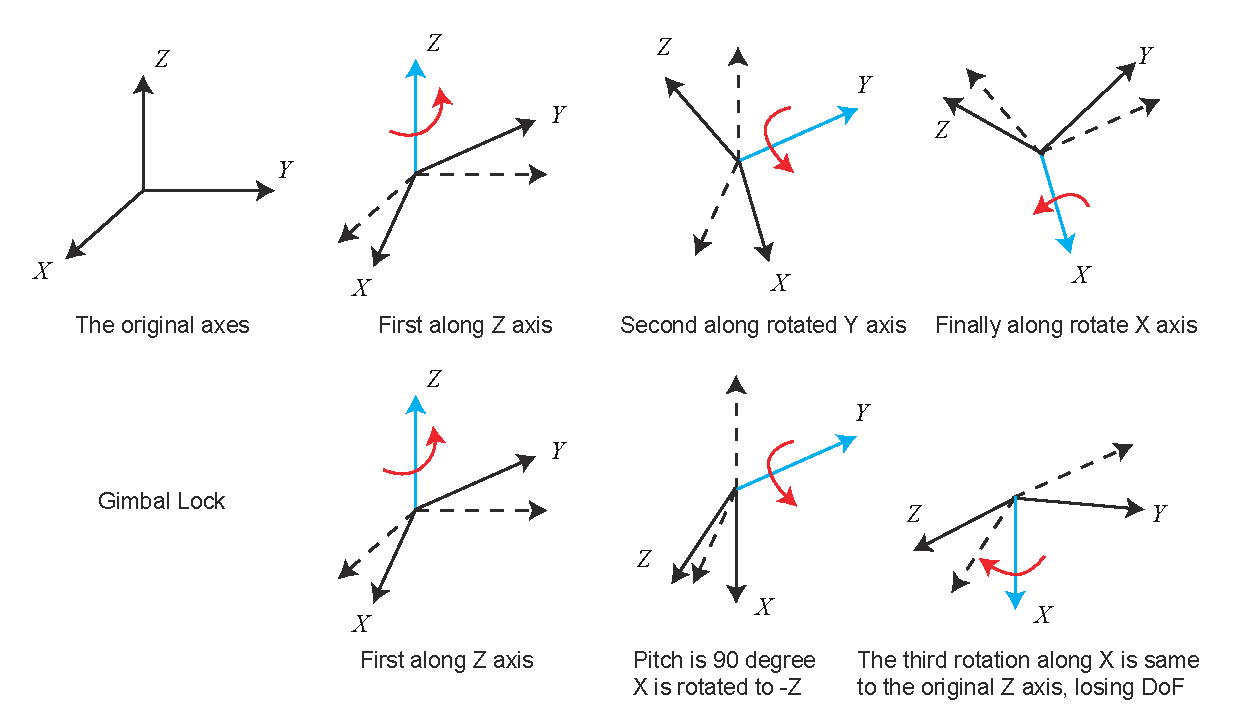
\includegraphics[width=1.0\textwidth]{rigidMotion/eulerAngles.pdf}
	\caption{欧拉角的旋转示意图。上方为ZYX角定义。下方为pitch=$90^\circ$时,第三次旋转与第一次滚转角相同,使得系统丢失了一个自由度。如果你还没有理解万向锁,可以看看相关视频,理解起来会更方便。}
	\label{fig:eulerAngles}
\end{figure}

此时,可以使用$[r,p,y]^\mathrm{T}$这样一个三维的向量描述任意旋转。这个向量十分直观,我们可以从这个向量想象出旋转的过程。其他的欧拉角亦是通过这种方式,把旋转分解到3个轴上,得到一个三维的向量,只不过选用的轴及顺序不一样。这里介绍的rpy角是比较常用的一种,只有很少的欧拉角种类会有rpy这样脍炙人口的名字。不同的欧拉角是按照旋转轴的顺序来称呼的。例如,rpy角的旋转顺序是$ZYX$。同样,也有$XYZ, ZYZ$这样的欧拉角——但是它们就没有专门的名字了。值得一提的是,大部分领域在使用欧拉角时都有各自的坐标方向和顺序上的习惯,不一定和我们这里说的相同。

欧拉角的一个重大缺点是会碰到著名的\textbf{万向锁问题}(Gimbal Lock\footnote{\url{https://en.wikipedia.org/wiki/Gimbal_lock}。}):在俯仰角为$\pm 90 ^\circ $时,第一次旋转与第三次旋转将使用同一个轴,使得系统丢失了一个自由度(由3次旋转变成了2次旋转)。这被称为奇异性问题,在其他形式的欧拉角中也同样存在。理论上可以证明,只要想用3个实数来表达三维旋转时,都会不可避免地碰到奇异性问题\footnote{旋转向量也有奇异性,发生在转角$\theta$超过$2\pi$而产生周期性时。}。由于这种原理,欧拉角不适于插值和迭代,往往只用于人机交互中。我们也很少在SLAM程序中直接使用欧拉角表达姿态,同样不会在滤波或优化中使用欧拉角表达旋转(因为它具有奇异性)。不过,若你想验证自己的算法是否有错,转换成欧拉角能够帮你快速分辨结果是否正确。在某些主体主要为2D运动的场合(例如扫地机、自动驾驶车辆),我们也可以把旋转分解成三个欧拉角,然后把其中一个(例如偏航角)拿出来作为定位信息输出。

\section{四元数}
\subsection{四元数的定义}
旋转矩阵用9个量描述3自由度的旋转,具有冗余性;欧拉角和旋转向量是紧凑的,但具有奇异性。事实上,我们\textbf{找不到不带奇异性的三维向量描述方式}\textsuperscript{\cite{Stuelpnagel1964}}。这有点类似于用两个坐标表示地球表面(如经度和纬度),将必定存在奇异性(纬度为$\pm 90^\circ$时经度无意义)。

回忆以前学习过的复数。我们用复数集$\mathbb{C}$表示复平面上的向量,而复数的乘法则表示复平面上的旋转:例如,乘上复数$i$相当于逆时针把一个复向量旋转$90^\circ$。类似地,在表达三维空间旋转时,也有一种类似于复数的代数:\textbf{四元数}(Quaternion)。四元数是Hamilton找到的一种扩展的复数。它\textbf{既是紧凑的,也没有奇异性}。如果说缺点,四元数不够直观,其运算稍复杂些。

把四元数与复数类比可以帮助你更快地理解四元数。例如,当我们想要将复平面的向量旋转$\theta$角时,可以给这个复向量乘以$\mathrm{e}^{i\theta}$。这是极坐标表示的复数,它也可以写成普通的形式,只要使用欧拉公式即可:
\begin{equation}
\mathrm{e}^{i\theta} = \cos \theta + i \sin \theta.
\end{equation}
这正是一个单位长度的复数。所以,在二维情况下,旋转可以由\textbf{单位复数}来描述。类似地,我们会看到,三维旋转则可以由\textbf{单位四元数}来描述。

一个四元数$\bm{q}$拥有一个实部和三个虚部。本书把实部写在前面(也有地方把实部写在后面),像下面这样:
\begin{equation}
 \bm{q} = q_0 + q_1 i + q_2 j + q_3 k,
\end{equation}
其中$i,j,k$为四元数的三个虚部。这三个虚部满足以下关系式:
\begin{equation}
\label{eq:quaternionVirtual}
\left\{ \begin{array}{l}
{i^2} = {j^2} = {k^2} =  - 1\\
ij = k,ji =  - k\\
jk = i,kj =  - i\\
ki = j,ik =  - j
\end{array} \right. .
\end{equation}
如果把$i,j,k$看成三个坐标轴,那么它们与自己的乘法和复数一样,相互之间的乘法和外积一样。有时人们也用一个标量和一个向量来表达四元数:
\[
 \bm{q} = \left[ s, \bm{v} \right]^\mathrm{T}, \quad s=q_0 \in \mathbb{R},\quad \bm{v} = [q_1, q_2, q_3]^\mathrm{T} \in \mathbb{R}^3,
\]
这里,$s$称为四元数的实部,而$\bm{v}$称为它的虚部。如果一个四元数的虚部为$\bm{0}$,称之为\textbf{实四元数}。反之,若它的实部为$0$,则称之为\textbf{虚四元数}。

%考虑到三维空间需要3个轴,四元数也有3个虚部,那么,一个虚四元数能不能对应到一个空间点呢?事实上我们就是这样做的。

可以用\textbf{单位四元数}表示三维空间中任意一个旋转,不过这种表达方式和复数有着微妙的不同。在复数中,乘以$i$意味着旋转$90^\circ$。这是否意味着四元数中,乘$i$就是绕$i$轴旋转$90^\circ$?那么,$ij=k$是否意味着,先绕$i$转$90^\circ$,再绕$j$转$90^\circ$,就等于绕$k$转$90^\circ$?读者可以找一部手机比划一下——然后你会发现情况并不是这样。正确的情形应该是,乘以$i$对应着旋转$180^\circ$,这样才能保证$ij=k$的性质。而$i^2=-1$,意味着绕$i$轴旋转$360^\circ$后得到一个相反的东西。这个东西要旋转两周才会和它原先的样子相等。

这似乎有些玄妙了,完整的解释需要引入太多额外的东西,我们还是冷静一下回到眼前。至少,我们知道单位四元数能够表达三维空间的旋转。那么四元数本身有些什么性质,它们互相之间又可以做哪些运算呢?下面我们先考察四元数之间的运算法则。

\subsection{四元数的运算}
四元数和通常复数一样,可以进行一系列的运算。常见的有四则运算、数乘、求逆、共轭等。下面分别介绍。

现有两个四元数$\bm{q}_a, \bm{q}_b$,它们的向量表示为$[s_a, \bm{v}_a]^\mathrm{T}, [s_b, \bm{v}_b]^\mathrm{T}$,或者原始四元数表示为:
\[
\bm{q}_a = s_a+x_ai+y_aj+z_ak, \quad \bm{q}_b  = s_b+x_bi+y_bj+z_bk.
\]
那么,其运算可表示如下。

\begin{enumerate}
	\item {\emph{加法和减法}}
	
	四元数$\bm{q}_a, \bm{q}_b$的加减运算为:
	\begin{equation} 	
	\bm{q}_a \pm \bm{q}_b = \left[ s_a \pm s_b, \bm{v}_a \pm \bm{v}_b \right]^\mathrm{T}.
	\end{equation}
	\item{\emph{乘法}}
	
	乘法是把$\bm{q}_a$的每一项与$\bm{q}_b$的每项相乘,最后相加,虚部要按照式\eqref{eq:quaternionVirtual}进行。整理可得:
	\begin{equation}
	\begin{aligned}
	\bm{q}_a \bm{q}_b &= {s_a}{s_b} - {x_a}{x_b} - {y_a}{y_b} - {z_a}{z_b}\\
	&+ \left( {{s_a}{x_b} + {x_a}{s_b} + {y_a}{z_b} - {z_a}{y_b}} \right)i\\
	&+ \left( {{s_a}{y_b} - {x_a}{z_b} + {y_a}{s_b} + {z_a}{x_b}} \right)j\\
	&+ \left( {{s_a}{z_b} + {x_a}{y_b} - {y_a}{x_b} + {z_a}{s_b}} \right)k.
	\end{aligned}
	\end{equation}
	虽然稍为复杂,但形式上是整齐有序的。如果写成向量形式并利用内外积运算,该表达会更加简洁:
	\begin{equation}
	\bm{q}_a \bm{q}_b = \left[ s_a s_b - \bm{v}_a^\mathrm{T} \bm{v}_b, s_a\bm{v}_b + s_b\bm{v}_a + \bm{v}_a \times \bm{v}_b \right]^\mathrm{T}.
	\end{equation}
	在该乘法定义下,两个实的四元数乘积仍是实的,这与复数也是一致的。然而,注意到,由于最后一项外积的存在,四元数乘法通常是不可交换的,除非$\bm{v}_a$和$\bm{v}_b$在$\mathbb{R}^3$中共线,此时外积项为零。

	\item { \emph{模长} }
		
	四元数的模长定义为
	\begin{equation}
	\| \bm{q}_a \| = \sqrt{ s_a^2 + x_a^2 + y_a^2 + z_a^2 }.
	\end{equation}
	可以验证,两个四元数乘积的模即为模的乘积。这使得单位四元数相乘后仍是单位四元数。
	\begin{equation}
	\| \bm{q}_a \bm{q}_b \| = \|\bm{q}_a \| \| \bm{q}_b \|.
	\end{equation}
	
	\item { \emph{共轭} }
	
	四元数的共轭是把虚部取成相反数:
	\begin{equation}
	\bm{q}_a^* = s_a - x_ai - y_aj - z_ak = [s_a, -\bm{v}_a]^\mathrm{T}.
	\end{equation}
	四元数共轭与其本身相乘,会得到一个实四元数,其实部为模长的平方:
	\begin{equation}
	\bm{q}^* \bm{q} = \bm{q} \bm{q}^* = [s_a^2+\bm{v}^\mathrm{T} \bm{v}, \bm{0} ]^\mathrm{T}.
	\end{equation}

	\item{ \emph{逆} }
	
	一个四元数的逆为
	\begin{equation}
	\label{eq:quaternionInverse}
	\bm{q}^{-1} = \bm{q}^* / \| \bm{q} \| ^2.
	\end{equation}
	按此定义,四元数和自己的逆的乘积为实四元数$\bm{1}$:
	\begin{equation}
	\bm{q} \bm{q}^{-1} = \bm{q}^{-1} \bm{q} = \bm{1}.
	\end{equation}
	
	如果$\bm{q}$为单位四元数,其逆和共轭就是同一个量。同时,乘积的逆有和矩阵相似的性质:
	\begin{equation}
	\left( \bm{q}_a \bm{q}_b \right)^{-1} = \bm{q}_b^{-1} \bm{q}_a^{-1}.
	\end{equation}
	
	\item{ \emph{数乘} }
	
	和向量相似,四元数可以与数相乘:
	\begin{equation}
	k \bm{q} = \left[ ks, k\bm{v} \right]^\mathrm{T}.
	\end{equation}
\end{enumerate}

\subsection{用四元数表示旋转}
我们可以用四元数表达对一个点的旋转。假设一个空间三维点$\bm{p} = [x,y,z]\in \mathbb{R}^3$,以及一个由单位四元数$\bm{q}$指定的旋转。三维点$\bm{p}$经过旋转之后变为$\bm{p}'$。如果使用矩阵描述,那么有$\bm{p}'=\bm{R} \bm{p}$。而如果用四元数描述旋转,它们的关系又如何来表达呢?

首先,把三维空间点用一个虚四元数来描述:
\[
\bm{p} = [0, x, y, z]^\mathrm{T} = [0, \bm{v}]^\mathrm{T}. 
\]
相当于把四元数的3个虚部与空间中的3个轴相对应。那么,旋转后的点$\bm{p}'$即可表示为这样的乘积:
\begin{equation}\label{eq:rotate-with-quaternion}
\bm{p}' = \bm{q} \bm{p} \bm{q}^{-1}.
\end{equation}
这里的乘法均为四元数乘法,结果也是四元数。最后把$\bm{p}'$的虚部取出,即得旋转之后点的坐标。并且,可以验证(留作习题),计算结果的实部为0,故为纯虚四元数。

\subsection{四元数到其他旋转表示的转换}
任意单位四元数描述了一个旋转,该旋转亦可用旋转矩阵或旋转向量描述。现在来考察四元数与旋转向量、旋转矩阵之间的转换关系。在此之前,我们要说,四元数乘法也可以写成一种矩阵的乘法。设$\bm{q}=[s,\bm{v}]^\mathrm{T}$,那么,定义如下的符号$^{+}$和$^{\oplus}$为\textsuperscript{\cite{Barfoot2011}}:
\begin{equation}
\bm{q}^{+}=\left[\begin{array}{cc}
s&-\bm{v}^\mathrm{T} \\
\bm{v}&s\bm{I}+\bm{v}^{\wedge}
\end{array}\right],\quad 
\bm{q}^{\oplus}=
\left[\begin{array}{cc}
s & -\bm{v}^\mathrm{T} \\
\bm{v} & s\bm{I}-\bm{v}^{\wedge}
\end{array}\right],
\end{equation}
这两个符号将四元数映射成为一个4$\times$4的矩阵。于是四元数乘法可以写成矩阵的形式:
\begin{equation}
\bm{q}_1^ + {\bm{q}_2} = \left[ {\begin{array}{*{20}{c}}
	s_1&-\bm{v}_1^T\\
	\bm{v}_1 & s_1 \bm{I} + \bm{v}_1^\wedge
	\end{array}} \right]\left[ {\begin{array}{*{20}{c}}
	{{s _2}} \\
	{{\bm{v} _2}}
	\end{array}} \right] = \left[ {\begin{array}{*{20}{c}}
	{ - \bm{v} _1^T{\bm{v} _2} + {s _1}{s _2}} \\ 
	{{s _1}{\bm{v} _2} + {s _2}{\bm{v} _1} + \bm{v} _1^ \wedge {\bm{v} _2}}
	\end{array}} \right] = \bm{q}_1 \bm{q}_2
\end{equation}
同理亦可证:
\begin{equation}
\bm{q}_1 \bm{q}_2 = \bm{q}_1^{+} \bm{q}_2 = \bm{q}_2^{\oplus} \bm{q}_1.
\end{equation}

然后,考虑使用四元数对空间点进行旋转的问题。根据前面的说法,有:
\begin{equation}
\begin{split}
\bm{p}' &= \bm{q} \bm{p} \bm{q}^{-1} = \bm{q}^+ \bm{p}^+ \bm{q}^{-1} \\
&= \bm{q}^+ \bm{q}^{{-1}^{\oplus}} \bm{p}.
\end{split}
\end{equation}
代入两个符号对应的矩阵,得:
\begin{equation}\label{eq:quaternion-to-rotation-matrix-derive}
{\bm{q}^ + }{\left( {{\bm{q}^{ - 1}}} \right)^ \oplus } = \left[ \begin{array}{*{20}{c}}
	s&-\bm{v}^T\\
	\bm{v}&s\bm{I}+\bm{v}^\wedge 
	\end{array} \right]\left[\begin{array}{*{20}{c}}
	s&{\bm{v} ^T}\\
	{ - \bm{v} }&{s\bm{I} + \bm{v} ^ \wedge }
	\end{array} \right] = \left[ \begin{array}{*{20}{c}}
	1&\bm{0} \\
	\bm{0}^\mathrm{T}&\bm{v}\bm{v}^\mathrm{T} + {s^2} \bm{I} + 2s\bm{v} ^ \wedge + {(\bm{v} ^ \wedge)}^2 
	\end{array} \right].
\end{equation}
因为$\bm{p}'$和$\bm{p}$都是虚四元数,那么事实上该矩阵的右下角即给出了\textbf{从四元数到旋转矩阵}的变换关系:
\begin{equation}
\bm{R} = \bm{v} \bm{v}^\mathrm{T} + {s^2} \bm{I} + 2s\bm{v} ^ \wedge + {(\bm{v} ^ \wedge)}^2.
\end{equation}
为了得到四元数到旋转向量的转换公式,对上式两侧求迹,得:
\begin{equation}
\begin{aligned}
\mathrm{tr}(\bm{R}) &= \mathrm{tr}(\bm{v}\bm{v}^\mathrm{T} + 3s^2 + 2s \cdot 0 + \mathrm{tr}((\bm{v}^\wedge)^2) \\
&= v_1^2+v_2^2+v_3s^2 + 3s^2 - 2(v_1^2+v_2^2+v_3^2) \\
&= (1-s^2) + 3s^2 -2(1-s^2)\\
&= 4s^2 -1.
\end{aligned}
\end{equation}
又由式\eqref{eq:R2theta}得:
\begin{equation}
\begin{aligned}
\theta &= \arccos(\frac{\mathrm{tr}(\bm{R}-1)}{2}) \\
&=\arccos(2s^2-1).
\end{aligned}
\end{equation}
即
\begin{equation}
\cos \theta =2s^2-1=2 \cos^2 \frac{\theta}{2} -1,
\end{equation}
所以:
\begin{equation}
\theta = 2 \arccos s.
\end{equation}
至于旋转轴,如果在式\eqref{eq:quaternion-to-rotation-matrix-derive}中用$\bm{q}$的虚部代替$\bm{p}$,易知$\bm{q}$的虚部组成的向量在旋转时是不动的,即构成旋转轴。于是只要将它除掉它的模长,即得。总而言之,四元数到旋转向量的转换公式可列写如下:
\begin{equation}
\label{eq:rotationVector2Quaternion}
\begin{cases}
\theta  = 2\arccos {q_0}\\
{\left[ {{n_x},{n_y},{n_z}} \right]^\mathrm{T}} = {{{\left[ {{q_1},{q_2},{q_3}} \right]}^\mathrm{T}}}/{\sin \frac{\theta }{2}}
\end{cases} .
\end{equation}

至于如何从其他方式转换到四元数,只须把上述步骤倒过来处理即可。在实际编程中,程序库通常会为我们准备好各种形式之间的转换。无论是四元数、旋转矩阵还是轴角,它们都可以用来描述同一个旋转。我们应该在实际中选择最为方便的形式,而不必拘泥于某种特定的形式。在随后的实践和习题中,我们会演示各种表达方式之间的转换,以加深读者的印象。


%
%从旋转向量到四元数的转换方式已在式\eqref{eq:rotationVector2Quaternion}中给出。因此,现在看来把四元数转换为矩阵的最直观方法,是先把四元数$\bm{q}$转换为轴角$\theta$和$\bm{n}$,然后再根据罗德里格斯公式转换为矩阵。不过那样要计算一个$\arccos$函数,代价较大。实际上这个计算是可以通过一定的技巧绕过的。这里省略推导过程,直接给出四元数到旋转矩阵的转换方式。
%
%这种表达方式和旋转矩阵、旋转向量有什么关系呢?我们不妨先来看旋转向量。假设某个旋转是绕单位向量$\bm{n}=\left[ n_x, n_y, n_z \right]^\mathrm{T}$进行了角度为$\theta$的旋转,那么这个旋转的四元数形式为
%\begin{equation}
%\label{eq:ntheta2quaternion}
%\bm{q} = \left[ \cos \frac{\theta}{2}, n_x \sin \frac{\theta}{2}, n_y \sin \frac{\theta}{2}, n_z \sin \frac{\theta}{2}\right]^\mathrm{T} .
%\end{equation}
%
%反之,亦可从单位四元数中计算出对应旋转轴与夹角:
%
%
%这个式子给了我们一种微妙的“转了一半”的感觉。同样,对式\eqref{eq:ntheta2quaternion}的$\theta$加上$2\pi$,我们得到一个相同的旋转,但此时对应的四元数变成了$-\bm{q}$。因此,在四元数中,\textbf{任意的旋转都可以由两个互为相反数的四元数表示}。同理,取$\theta$为$0$,则得到一个没有任何旋转的实四元数:
%\begin{equation}
%\bm{q}_0 = \left[ { \pm 1,0,0,0} \right]^\mathrm{T} .
%\end{equation}
%
%设四元数$\bm{q} = q_0+q_1i+q_2j+q_3k$,对应的旋转矩阵$\bm{R}$为
%\begin{equation}
%\bm{R} = \left[ {\begin{array}{*{20}{c}}
%	 {1 - 2q_2^2 - 2q_3^2}&{2{q_1}{q_2} - 2{q_0}{q_3}}&{2{q_1}{q_3} + 2{q_0}{q_2}}\\
%	 {2{q_1}{q_2} + 2{q_0}{q_3}}&{1 - 2q_1^2 - 2q_3^2}&{2{q_2}{q_3} - 2{q_0}{q_1}}\\
%	 {2{q_1}{q_3} - 2{q_0}{q_2}}&{2{q_2}{q_3} + 2{q_0}{q_1}}&{1 - 2q_1^2 - 2q_2^2}
% \end{array}} \right].
%\end{equation}
%
%反之,由旋转矩阵到四元数的转换如下。假设矩阵为$\bm{R}=\{ m_{ij}\}, i, j \in \left[ 1, 2,3 \right] $,其对应的四元数$\bm{q}$由下式给出:
%\begin{equation}
%{q_0} = \frac{{\sqrt {\mathrm{tr}(R) + 1} }}{2},{q_1} = \frac{{{m_{23}} - {m_{32}}}}{{4{q_0}}},{q_2} = \frac{{{m_{31}} - {m_{13}}}}{{4{q_0}}},{q_3} = \frac{{{m_{12}} - {m_{21}}}}{{4{q_0}}}.
%\end{equation}
%
%值得一提的是,由于$\bm{q}$和$\bm{-q}$表示同一个旋转,事实上一个$\bm{R}$对应的四元数表示并不是唯一的。同时,除了上面给出的转换方式之外,还存在其他几种计算方法,而本书都省略了。实际编程中,当$q_0$接近0时,其余3个分量会非常大,导致解不稳定,此时我们再考虑使用其他的方式进行转换。

\section{\textsuperscript{\ttfamily *}相似、仿射、射影变换}
除了欧氏变换之外,3D空间还存在其他几种变换方式,只不过欧氏变换是最简单的。它们一部分和测量几何有关,因为在之后的讲解中可能会提到,所以先罗列出来。欧氏变换保持了向量的长度和夹角,相当于我们把一个刚体原封不动地进行了移动或旋转,不改变它自身的样子。其他几种变换则会改变它的外形。它们都拥有类似的矩阵表示。

\begin{enumerate}
	\item {\emph{相似变换}}
	
	相似变换比欧氏变换多了一个自由度,它允许物体进行均匀缩放,其矩阵表示为
	\begin{equation}
	\bm{T}_S = \left[ {\begin{array}{*{20}{c}}
		{s \bm{R}}& \bm{t}\\
		{{ \bm{0}^\mathrm{T}}}&1
		\end{array}} \right].
	\end{equation}
	
	注意到旋转部分多了一个缩放因子$s$,表示我们在对向量旋转之后,可以在$x,y,z$三个坐标上进行均匀缩放。由于含有缩放,相似变换不再保持图形的面积不变。你可以想象一个边长为1的立方体通过相似变换后,变成边长为10的样子(但仍然是立方体)。三维相似变换的集合也叫做\textbf{相似变换群},记作$\mathrm{Sim}(3)$。
	
	\item { \emph{仿射变换} }
	
	仿射变换的矩阵形式如下:
	\begin{equation}
	\bm{T}_A = \left[ {\begin{array}{*{20}{c}}
		\bm{A} & \bm{t}\\
		{{\bm{0}^\mathrm{T}}} & 1
		\end{array}} \right].
	\end{equation}
	
	与欧氏变换不同的是,仿射变换只要求$\bm{A}$是一个可逆矩阵,而不必是正交矩阵。仿射变换也叫正交投影。经过仿射变换之后,立方体就不再是方的了,但是各个面仍然是平行四边形。
	
	\item{ \emph{射影变换} }
	
	射影变换是最一般的变换,它的矩阵形式为
	
	\begin{equation}
	{\bm{T}_P} = \left[ {\begin{array}{*{20}{c}}
		\bm{A} & \bm{t}\\
		{{\bm{a}^\mathrm{T}}} & v
		\end{array}} \right].
	\end{equation}
	
	它的左上角为可逆矩阵$\bm{A}$,右上角为平移$\bm{t}$,左下角为缩放$\bm{a}^\mathrm{T}$。由于采用了齐次坐标,当$v \neq 0$时,我们可以对整个矩阵除以$v$得到一个右下角为1的矩阵; 否则得到右下角为$0$的矩阵。因此,2D的射影变换一共有8个自由度,3D则共有15个自由度。射影变换是现在讲过的变换中,形式最为一般的。从真实世界到相机照片的变换可以看成一个射影变换。读者可以想象一个原本方形的地板砖,在照片当中是什么样子:首先,它不再是方形的。由于近大远小的关系,它甚至不是平行四边形,而是一个不规则的四边形。
\end{enumerate}

\autoref{table:common-transform}总结了目前讲到的几种变换的性质。注意在“不变性质”中,从上到下是有包含关系的。例如,欧氏变换除了保体积之外,也具有保平行、相交等性质。

\begin{table}[!htp]
	\centering
	\caption{常见变换性质比较}
	\label{table:common-transform}
	\begin{tabu}{c|c|c|c}
		\toprule
		变换名称 & 矩阵形式 & 自由度 & 不变性质 \\ \midrule
		欧氏变换 \rule{0pt}{20 pt} & $\left[ {\begin{array}{*{20}{c}}
			\bm{R} & \bm{t}\\
			{{\bm{0}^\mathrm{T}}}&1
			\end{array}} \right]$ & 6 & 长度、夹角、体积 \\ 
		相似变换 \rule{0pt}{20 pt}& $ \left[ {\begin{array}{*{20}{c}}
			{s \bm{R}}& \bm{t}\\
			{{ \bm{0}^\mathrm{T}}}&1
			\end{array}} \right]$ & 7 & 体积比 \\ 
		仿射变换 \rule{0pt}{20 pt}& $ \left[ {\begin{array}{*{20}{c}}
			\bm{A} & \bm{t}\\
			{{\bm{0}^\mathrm{T}}} & 1
			\end{array}} \right]$   & 12 & 平行性、体积比 \\ 
		射影变换 \rule{0pt}{20 pt} & $ \left[ {\begin{array}{*{20}{c}}
			\bm{A} & \bm{t}\\
			{{\bm{a}^\mathrm{T}}} & v
			\end{array}} \right]$ & 15 & 接触平面的相交和相切 \rule{0pt}{20 pt}\\ 
		\bottomrule
	\end{tabu} 
\end{table}

我们之后会说到,从真实世界到相机照片的变换是一个射影变换。如果相机的焦距为无穷远,那么这个变换为仿射变换。不过,在详细讲述相机模型之前,我们只要对它们有个大致的印象即可。

\section{实践:Eigen几何模块}
\subsection{Eigen几何模块的数据演示}
现在,我们来实际演练一下前面讲到的各种旋转表达方式。我们将在Eigen中使用四元数、欧拉角和旋转矩阵,演示它们之间的变换方式。我们还会给出一个可视化程序,帮助读者理解这几个变换的关系。

\begin{lstlisting}[language=c++,caption=slambook2/ch3/useGeometry/useGeometry.cpp]
#include <iostream>
#include <cmath>
using namespace std;

#include <Eigen/Core>
#include <Eigen/Geometry>

using namespace Eigen;
// 本程序演示了 Eigen 几何模块的使用方法

int main(int argc, char **argv) {
    // Eigen/Geometry 模块提供了各种旋转和平移的表示
    // 3D 旋转矩阵直接使用 Matrix3d 或 Matrix3f
    Matrix3d rotation_matrix = Matrix3d::Identity();
    // 旋转向量使用 AngleAxis, 它底层不直接是Matrix,但运算可以当作矩阵(因为重载了运算符)
    AngleAxisd rotation_vector(M_PI / 4, Vector3d(0, 0, 1));     //沿 Z 轴旋转 45 度
    cout.precision(3);
    cout << "rotation matrix =\n" << rotation_vector.matrix() << endl;   //用matrix()转换成矩阵
    // 也可以直接赋值
    rotation_matrix = rotation_vector.toRotationMatrix();
    // 用 AngleAxis 可以进行坐标变换
    Vector3d v(1, 0, 0);
    Vector3d v_rotated = rotation_vector * v;
    cout << "(1,0,0) after rotation (by angle axis) = " << v_rotated.transpose() << endl;
    // 或者用旋转矩阵
    v_rotated = rotation_matrix * v;
    cout << "(1,0,0) after rotation (by matrix) = " << v_rotated.transpose() << endl;
    
    // 欧拉角: 可以将旋转矩阵直接转换成欧拉角
    Vector3d euler_angles = rotation_matrix.eulerAngles(2, 1, 0); // ZYX顺序,即roll pitch yaw顺序
    cout << "yaw pitch roll = " << euler_angles.transpose() << endl;
    
    // 欧氏变换矩阵使用 Eigen::Isometry
    Isometry3d T = Isometry3d::Identity();       // 虽然称为3d,实质上是4*4的矩阵
    T.rotate(rotation_vector);                   // 按照rotation_vector进行旋转
    T.pretranslate(Vector3d(1, 3, 4));           // 把平移向量设成(1,3,4)
    cout << "Transform matrix = \n" << T.matrix() << endl;
    
    // 用变换矩阵进行坐标变换
    Vector3d v_transformed = T * v;                              // 相当于R*v+t
    cout << "v tranformed = " << v_transformed.transpose() << endl;
    
    // 对于仿射和射影变换,使用 Eigen::Affine3d 和 Eigen::Projective3d 即可,略
    
    // 四元数
    // 可以直接把AngleAxis赋值给四元数,反之亦然
    Quaterniond q = Quaterniond(rotation_vector);
    cout << "quaternion from rotation vector = " << q.coeffs().transpose()
    << endl;   // 请注意coeffs的顺序是(x,y,z,w),w为实部,前三者为虚部
    // 也可以把旋转矩阵赋给它
    q = Quaterniond(rotation_matrix);
    cout << "quaternion from rotation matrix = " << q.coeffs().transpose() << endl;
    // 使用四元数旋转一个向量,使用重载的乘法即可
    v_rotated = q * v; // 注意数学上是qvq^{-1}
    cout << "(1,0,0) after rotation = " << v_rotated.transpose() << endl;
    // 用常规向量乘法表示,则应该如下计算
    cout << "should be equal to " << (q * Quaterniond(0, 1, 0, 0) * q.inverse()).coeffs().transpose() << endl;
    
    return 0;
}
\end{lstlisting}

Eigen中对各种形式的表达方式总结如下。请注意每种类型都有单精度和双精度两种数据类型,而且和之前一样,不能由编译器自动转换。下面以双精度为例,你可以把最后的d改成f,即得到单精度的数据结构。
\begin{itemize}
	\item 旋转矩阵($3 \times 3$):Eigen::Matrix3d。
	\item 旋转向量($3 \times 1$):Eigen::AngleAxisd。
	\item 欧拉角($3 \times 1$):Eigen::Vector3d。
	\item 四元数($4 \times 1$):Eigen::Quaterniond。
	\item 欧氏变换矩阵($4 \times 4$):Eigen::Isometry3d。
	\item 仿射变换($4 \times 4$):Eigen::Affine3d。
	\item 射影变换($4 \times 4$):Eigen::Projective3d。
\end{itemize}

参考代码中对应的CMakeLists即可编译此程序。在这个程序中,演示了如何使用Eigen中的旋转矩阵、旋转向量(AngleAxis)、欧拉角和四元数。我们用这几种旋转方式去旋转一个向量$\bm{v}$,发现结果是一样的(不一样就真是见鬼了)。同时,也演示了如何在程序中转换这几种表达方式。想进一步了解Eigen的几何模块的读者可以参考(\url{http://eigen.tuxfamily.org/dox/group__TutorialGeometry.html})。

请读者注意,\textbf{程序代码通过和数学表示有一些细微的差别}。例如,通过运算符重载,四元数和三维向量可以直接计算乘法,但在数学上则需要先把向量转成虚四元数,再利用四元数乘法进行计算,同样的情况也适用于变换矩阵乘三维向量的情况。总体而言,程序中的用法会比数学公式更灵活一些。

\subsection{实际的坐标变换例子}
下面我们举一个小例子来演示坐标变换。

\noindent \textbf{例子} \quad \emph{设有小萝卜一号和小萝卜二号位于世界坐标系中。记世界坐标系为$W$,小萝卜们的坐标系为$R_1$和$R_2$。小萝卜一号的位姿为$\bm{q}_1 = [ 0.35, 0.2, 0.3, 0.1 ]^\mathrm{T}, \bm{t}_1 = [0.3, 0.1, 0.1]^\mathrm{T}$。小萝卜二号的位姿为$\bm{q}_2 = [ -0.5, 0.4, -0.1, 0.2 ]^\mathrm{T}, \bm{t}_2 = [-0.1, 0.5, 0.3]^\mathrm{T}$。这里的$\bm{q}$和$\bm{t}$表达的是$\bm{T}_{R_k, W},k=1,2$,也就是世界坐标系到相机坐标系的变换关系。现在,小萝卜一号看到某个点在自身的坐标系下坐标为$\bm{p}_{R_1} = [0.5,0,0.2]^\mathrm{T}$,求该向量在小萝卜二号坐标系下的坐标。}

这是一个非常简单,但又具有代表性的例子。在实际场景中你经常需要在同一个机器人的不同部分,或者不同机器人之间转换坐标。下面我们书写一段程序来演示这个计算。

\begin{lstlisting}[language=c++,caption=slambook2/ch3/examples/coordinateTransform.cpp]
#include <iostream>
#include <vector>
#include <algorithm>
#include <Eigen/Core>
#include <Eigen/Geometry>

using namespace std;
using namespace Eigen;

int main(int argc, char** argv) {
    Quaterniond q1(0.35, 0.2, 0.3, 0.1), q2(-0.5, 0.4, -0.1, 0.2);
    q1.normalize();
    q2.normalize();
    Vector3d t1(0.3, 0.1, 0.1), t2(-0.1, 0.5, 0.3);
    Vector3d p1(0.5, 0, 0.2);
    
    Isometry3d T1w(q1), T2w(q2);
    T1w.pretranslate(t1);
    T2w.pretranslate(t2);
    
    Vector3d p2 = T2w * T1w.inverse() * p1;
    cout << endl << p2.transpose() << endl;
    return 0;
}
\end{lstlisting}

程序输出的答案是$[-0.0309731,0.73499,0.296108]^\mathrm{T}$,计算过程也十分简单,只需计算$$\bm{p}_{R_2} = \bm{T}_{R_2,W}\bm{T}_{W, R_1} \bm{p}_{R_1}$$即可。注意四元数使用之前需要归一化。

\section{可视化演示}
\subsection{显示运动轨迹}
如果你是第一次接触旋转和平移这些概念,可能会觉得它们形式看起来很复杂,因为毕竟每种表达方式都可以与其他方式互相转换,而转换公式有时还比较长。不过,虽然旋转矩阵、变换矩阵的数值可能不够直观,但我们可以很容易地把它们画在窗口里面。

本节我们演示两个可视化例子。首先,假设我们通过某种方式记录了一个机器人的运动轨迹,现在想把它画到一个窗口中。假设轨迹文件存储于trajectory.txt,每一行用下面的格式存储:$$\mathrm{time}, t_x, t_y, t_z, q_x, q_y, q_z, q_w,$$其中$\mathrm{time}$指该位姿的记录时间,$\bm{t}$为平移,$\bm{q}$为旋转四元数,均是以世界坐标系到机器人坐标系记录。下面我们从文件中读取这些轨迹,并显示到一个窗口中。原则上,如果只是谈论“机器人的位姿”,那么你可以使用$\bm{T}_{WR}$或者$\bm{T}_{RW}$,事实上它们也只差一个逆而已,意味着知道其中一个就可以很轻松地得到另一个。如果你想要存储\textbf{机器人的轨迹},那么你可以存储所有时刻的$\bm{T}_{WR}$或者$\bm{T}_{RW}$,这并没有太大的差别。

在画轨迹的时候,我们可以把“轨迹”画成一系列点组成的序列,这和我们想象中的“轨迹”比较相似。严格说来,这其实是\textbf{机器人(相机)坐标系的原点在世界坐标系中的坐标}。考虑机器人坐标系的原点,即$\bm{O}_{R}$,那么,此时的$\bm{O}_{W}$就是这个原点在世界坐标系下的坐标:
\begin{equation}
\bm{O}_{W} = \bm{T}_{WR} \bm{O}_R = \bm{t}_{WR}.
\end{equation}
这正是$\bm{T}_{WR}$的平移部分。因此,可以从$\bm{T}_{WR}$中直接看到\textbf{相机在何处},这也是我们说$\bm{T}_{WR}$更为直观的原因。因此,在可视化程序里,轨迹文件存储了$\bm{T}_{WR}$而不是$\bm{T}_{RW}$。

最后,我们需要一个支持3D绘图的程序库。有许多库都支持3D绘图,比如大家熟悉的matlab,python的matplotlib,OpenGL等。在linux中,一个常见的库是基于OpenGL的Pangolin库\footnote{\url{https://github.com/stevenlovegrove/Pangolin}},它在支持OpenGL的绘图操作基础之上还提供了一些GUI的功能。在第二版的书籍中,我们使用git的submodule功能来管理本书依赖的第三方库。读者可以进入3rdparty文件夹中直接安装所需的库,git保证了我和你使用的版本是一致的。

\begin{lstlisting}[language=c++,caption=slambook2/ch3/examples/plotTrajectory.cpp]
#include <pangolin/pangolin.h>
#include <Eigen/Core>
#include <unistd.h>

using namespace std;
using namespace Eigen;

// path to trajectory file
string trajectory_file = "./examples/trajectory.txt";

void DrawTrajectory(vector<Isometry3d, Eigen::aligned_allocator<Isometry3d>>);

int main(int argc, char **argv) {
    vector<Isometry3d, Eigen::aligned_allocator<Isometry3d>> poses;
    ifstream fin(trajectory_file);
    if (!fin) {
        cout << "cannot find trajectory file at " << trajectory_file << endl;
        return 1;
    }
    
    while (!fin.eof()) {
        double time, tx, ty, tz, qx, qy, qz, qw;
        fin >> time >> tx >> ty >> tz >> qx >> qy >> qz >> qw;
        Isometry3d Twr(Quaterniond(qw, qx, qy, qz));
        Twr.pretranslate(Vector3d(tx, ty, tz));
        poses.push_back(Twr);
    }
    cout << "read total " << poses.size() << " pose entries" << endl;
    
    // draw trajectory in pangolin
    DrawTrajectory(poses);
    return 0;
}

void DrawTrajectory(vector<Isometry3d, Eigen::aligned_allocator<Isometry3d>> poses) {
    // create pangolin window and plot the trajectory
    pangolin::CreateWindowAndBind("Trajectory Viewer", 1024, 768);
    glEnable(GL_DEPTH_TEST);
    glEnable(GL_BLEND);
    glBlendFunc(GL_SRC_ALPHA, GL_ONE_MINUS_SRC_ALPHA);
    
    pangolin::OpenGlRenderState s_cam(
    pangolin::ProjectionMatrix(1024, 768, 500, 500, 512, 389, 0.1, 1000),
    pangolin::ModelViewLookAt(0, -0.1, -1.8, 0, 0, 0, 0.0, -1.0, 0.0)
    );
    
    pangolin::View &d_cam = pangolin::CreateDisplay()
        .SetBounds(0.0, 1.0, 0.0, 1.0, -1024.0f / 768.0f)
        .SetHandler(new pangolin::Handler3D(s_cam));
    
    while (pangolin::ShouldQuit() == false) {
        glClear(GL_COLOR_BUFFER_BIT | GL_DEPTH_BUFFER_BIT);
        d_cam.Activate(s_cam);
        glClearColor(1.0f, 1.0f, 1.0f, 1.0f);
        glLineWidth(2);
        for (size_t i = 0; i < poses.size(); i++) {
            // 画每个位姿的三个坐标轴
            Vector3d Ow = poses[i].translation();
            Vector3d Xw = poses[i] * (0.1 * Vector3d(1, 0, 0));
            Vector3d Yw = poses[i] * (0.1 * Vector3d(0, 1, 0));
            Vector3d Zw = poses[i] * (0.1 * Vector3d(0, 0, 1));
            glBegin(GL_LINES);
            glColor3f(1.0, 0.0, 0.0);
            glVertex3d(Ow[0], Ow[1], Ow[2]);
            glVertex3d(Xw[0], Xw[1], Xw[2]);
            glColor3f(0.0, 1.0, 0.0);
            glVertex3d(Ow[0], Ow[1], Ow[2]);
            glVertex3d(Yw[0], Yw[1], Yw[2]);
            glColor3f(0.0, 0.0, 1.0);
            glVertex3d(Ow[0], Ow[1], Ow[2]);
            glVertex3d(Zw[0], Zw[1], Zw[2]);
            glEnd();
        }
        // 画出连线
        for (size_t i = 0; i < poses.size(); i++) {
            glColor3f(0.0, 0.0, 0.0);
            glBegin(GL_LINES);
            auto p1 = poses[i], p2 = poses[i + 1];
            glVertex3d(p1.translation()[0], p1.translation()[1], p1.translation()[2]);
            glVertex3d(p2.translation()[0], p2.translation()[1], p2.translation()[2]);
            glEnd();
        }
        pangolin::FinishFrame();
        usleep(5000);   // sleep 5 ms
    }
}
\end{lstlisting}

该程序演示了如何在Panglin中画出3D的位姿。我们用红、绿、蓝三种颜色画出每个位姿的三个坐标轴(实际上我们计算了各坐标轴的世界坐标),然后用黑色线将轨迹连起来。程序运行结果如\autoref{fig:trajectory}所示。

\begin{figure}[!htp]
    \centering
    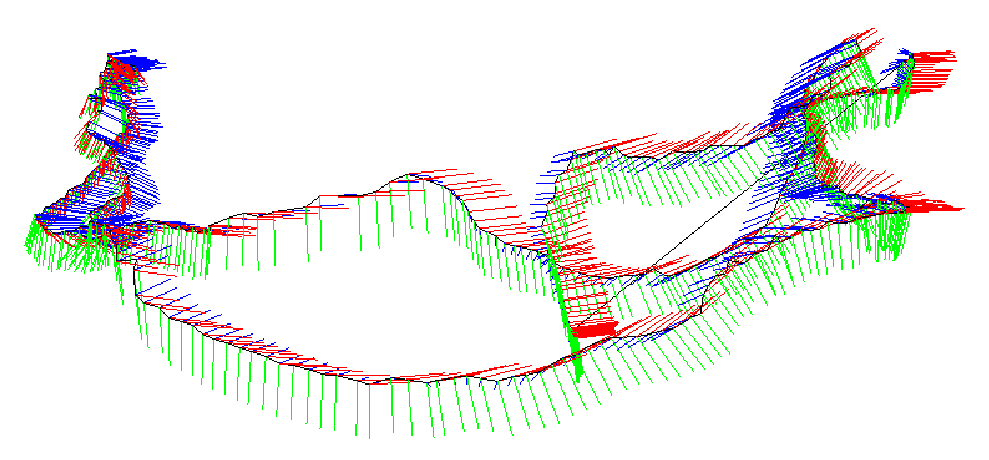
\includegraphics[width=0.8\textwidth]{rigidMotion/trajectory.pdf}
    \caption{位姿可视化的结果}
    \label{fig:trajectory}
\end{figure}

\subsection{显示相机的位姿}
\begin{figure}[!htp]
    \centering
    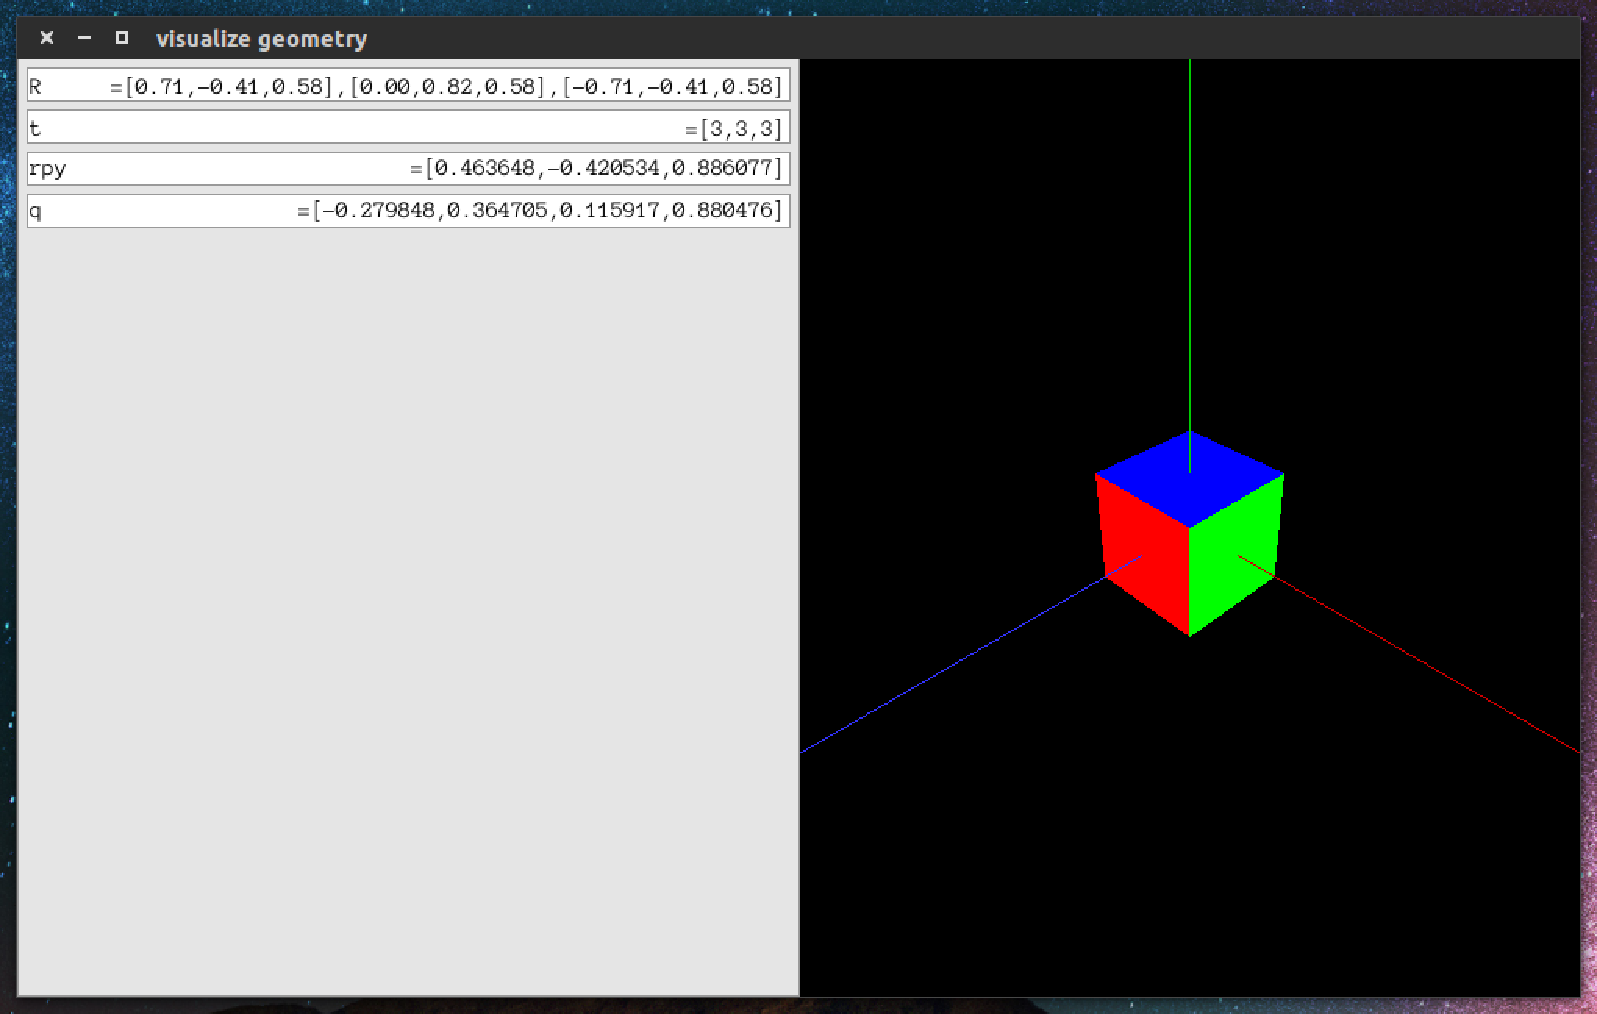
\includegraphics[width=0.8\textwidth]{rigidMotion/visualizeGeometry.pdf}
    \caption{旋转矩阵、欧拉角、四元数的可视化程序。}
    \label{fig:visualizeGeometry}
\end{figure}
除了显示轨迹之外,我们也可以显示3D窗口中相机的位姿。在slambook2/ch3/visualizeGeometry中,我们以可视化的形式演示了相机位姿的各种表达方式(见\autoref{fig:visualizeGeometry})。当读者用鼠标操作相机时,左侧的方框里会实时显示相机位姿对应的旋转矩阵、平移、欧拉角和四元数,你可以看看数据是如何变化的。根据我们的经验,除了欧拉角之外,你应该看不出它们直观的含义。然而,尽管旋转矩阵或变换矩阵并不直观,但是将它们可视化地显示出来并没有什么困难。该程序使用Pangolin库作为3D显示库,请参考Readme.txt来编译该程序。

\section*{习题}
\begin{enumerate}
	\item 验证旋转矩阵是正交矩阵。
	\item[\optional] 寻找罗德里格斯公式的推导过程并加以理解。
	\item 验证四元数旋转某个点后,结果是一个虚四元数(实部为零),所以仍然对应到一个三维空间点,见式\eqref{eq:rotate-with-quaternion}。
	\item 画表总结旋转矩阵、轴角、欧拉角、四元数的转换关系。
	\item 假设有一个大的Eigen矩阵,想把它的左上角$3 \times 3$的块取出来,然后赋值为$\bm{I}_{3 \times 3}$。请编程实现。
	\item[\optional] 一般线性方程$\bm{A} \bm{x}=\bm{b}$有哪几种做法?你能在Eigen中实现吗?
\end{enumerate}